% !TeX root = ../../Book1.tex
% 扩充编号：A09、A10。保测动力系统、平均遍历定理与逐点遍历定理。
% 初稿与必要自检不计正式审核；章末八题均为自拟训练题。
\OptionalChapter{时间平均与空间平均}{b1:ch:32}
\BookChapterNumber{b1:ch:32}

\begin{chapterabstract}
沿着同一条轨道反复观察并取平均，与在整个空间上积分，是两种不同的取平均方式。
保测性保证每次观察具有相同的总体分布，却还不能保证一条轨道代表整个空间。
本章先用不变事件描述轨道始终保留的信息，再从 Hilbert 空间的正交分解证明平均遍历定理，
并以极大不等式把容易计算的轨道平均推广到一般可积函数。
最终得到的极限是相对于不变信息的条件期望；遍历性恰好使这种条件平均化为常数。
圆周转动与倍增映射还将说明：平均能够稳定，并不意味着远隔时刻的相关性必然消失。
\end{chapterabstract}

\begin{learninggoals}
\begin{itemize}
\item\label{b1:item:32-goal-invariance}辨认保测变换与模零不变事件，解释不变子代数记录了什么信息，并用不变函数判别遍历性。
\item\label{b1:item:32-goal-hilbert}从 Hilbert 空间收缩算子的固定向量与算子差的值域出发，证明 von Neumann 平均遍历定理。
\item\label{b1:item:32-goal-maximal}掌握 Hopf 极大遍历引理及弱型估计，说明它们如何同时控制所有长度的平均误差。
\item\label{b1:item:32-goal-pointwise}把稠密类上的望远镜求和推广到一般可积函数，理解逐点极限的有限性、不变性及其与积分极限的关系。
\item\label{b1:item:32-goal-identification}把 Birkhoff 极限识别为相对于不变子代数的条件期望，区分遍历情形、非遍历情形及各种范数收敛。
\item\label{b1:item:32-goal-models}比较遍历性与混合性，完整分析无理圆周转动和二进倍增映射，并用它们检验平均结论的适用边界。
\end{itemize}
\end{learninggoals}

\chapref{b1:ch:30}研究独立随机变量的平均，\chapref{b1:ch:31}研究信息逐步增加时的条件平均。
本章更换了产生序列的方式：先固定一个变换 \(T\)，再观察
\(f(x),f(Tx),f(T^2x),\ldots\)。这些观测一般并不独立，也不自动构成鞅。
需要说明的是，变换保持测度这一整体条件，如何转化成单条轨道上平均值的稳定。

\ProseParagraphBreak

范数收敛与逐点收敛在这里解决不同的问题：前者控制整体的平均误差，后者描述一条给定轨道上的长期观察。Hilbert 空间的正交分解先解释哪些成分会被平均消去；极大估计再控制整段轨道上的误差。最后，条件期望把极限写成由不变信息决定的函数。

\ProseParagraphBreak

\secref{b1:sec:3201}先问哪些事件永远不能被变换混在一起，借此引入不变子代数和遍历性。
\secref{b1:sec:3202}暂时只问平均在 \(L^2\) 范数中是否收敛，
把函数空间分成“平均保留的部分”与“相邻两步相减的部分”。
这条算子论路线既给出一个完整的平均定理，也为后面的逐点逼近准备稠密类。

\ProseParagraphBreak

\secref{b1:sec:3203}用极大估计控制整条平均序列，
\secref{b1:sec:3204}则回答极限究竟是哪一个函数，并说明逐点收敛如何与 \(L^1\)、\(L^p\) 收敛衔接。
最后的\secref{b1:sec:3205}比较两个直观模型：无理转动使几乎处处的时间平均等于空间平均，
倍增映射还会使相隔很久的观测渐近失去相关。
读者应把“平均趋于常数”与“单次相关趋于乘积”作为两个不同的问题分别检查。

\ProseParagraphBreak

关于极大估计、逐点收敛及不变子代数，可对照 David H. Fremlin 的
《Measure Theory》\cite[372A--D, 372H--J]{Fremlin2016Measure}；
遍历性与混合性的函数判别见同书\cite[372O--Q]{Fremlin2016Measure}。
该书的部分论证放在一般算子或概率代数框架中。
本章讨论概率空间上的单个保测变换，先用 Hilbert 空间的正交分解建立稠密类，
再逐步证明极大估计、逐点收敛和条件期望的辨认。

% !TeX root = ../../Book1.tex
\section{保测变换与遍历性}
\label{b1:sec:3201}

设一个系统每过一个单位时间就由状态 \(x\) 变成 \(Tx\)。若 \(f(x)\) 表示在状态 \(x\) 观测到的温度、位置函数或某个事件的示性函数，那么沿一条轨道得到的数据是
\[
 f(x),\ f(Tx),\ f(T^2x),\ldots.
\]
把前 \(N\) 次观测相加后除以 \(N\)，得到时间平均。另一方面，若状态空间上给定概率测度 \(\mu\)，则 \(\int_X f\,\mathrm d\mu\) 描述按这一分布抽取状态时的空间平均。两种平均的取样方式不同；即使每个时刻的状态都服从同一分布，也不能直接断言一条轨道会代表整个空间。

\ProseParagraphBreak

本节先精确说明“分布不随时间改变”，再找出一条轨道始终无法离开的可测区域。如果空间可以分成几个互不交流、各有正测度的部分，长期平均就可能依赖初始状态落在哪一部分。后面出现的条件期望，正是相对于这部分不会被时间演化消除的信息取平均。

\subsection{保测变换与不变概率测度}
\label{b1:subsec:320101}

\begin{definition}\label{b1:def:measure-preserving-32}
设 \((X,\mathcal A,\mu)\) 是概率空间，\(T\colon X\rightarrow X\) 是 \(\mathcal A/\mathcal A\)-可测映射。如果对每个 \(A\in\mathcal A\) 都有
\begin{equation}\label{b1:eq:measure-preserving-32}
 \mu(T^{-1}A)=\mu(A),
\end{equation}
则称 \(T\) 是关于 \(\mu\) 的\term[baoce-bianhuan]{保测变换}[measure-preserving transformation]，也称 \(\mu\) 是 \(T\) 的\term[bubian-gailv-cedu]{不变概率测度}[invariant probability measure]。由概率空间和这个变换组成的 \((X,\mathcal A,\mu,T)\) 称为\term[baoce-dongli-xitong]{保测动力系统}[measure-preserving dynamical system]。
\end{definition}

这里 \(T^{-1}A\) 是集合的原像，不要求 \(T\) 有逆映射。式\eqref{b1:eq:measure-preserving-32}说的是：若初始状态按 \(\mu\) 分布，下一时刻落入 \(A\) 的概率，仍等于 \(\mu(A)\)。用推前测度的记号，这就是 \(T_\#\mu=\mu\)。不要把它改写成 \(\mu(TA)=\mu(A)\)：一般可测映射的像未必可测，即使像可测，后一个等式也未必成立。

\ProseParagraphBreak

保测性是 \(T\) 与 \(\mu\) 共同满足的条件。即使状态空间和变换已经固定，换一个概率测度也可能失去保测性。例如在两点集 \(X=\{a,b\}\) 上令 \(T\) 交换两点，则单点的概率必须相等；\(\mu(\{a\})=3/4\)、\(\mu(\{b\})=1/4\) 时，这个交换不保测。反过来，恒等映射关于每个概率测度都保测。因此保测还远不足以保证时间平均等于空间平均。

\ProseParagraphBreak

不变概率测度也可以是需要构造的对象。\cref{b1:prop:compact-invariant-probability}已经证明：
若 \(X\) 是非空紧致度量空间、\(T:X\to X\) 连续，
则轨道点质量的平均有弱收敛子列，其极限是一个不变 Borel 概率测度。
那一结论解决的是测度的存在，并不保证唯一性或遍历性。
本章从已经选定的保测概率系统出发，不要求一般可测空间具有紧性或拓扑。

\begin{proposition}[保测性的积分刻画]\label{b1:prop:preserving-integrals-32}
设 \((X,\mathcal A,\mu)\) 是概率空间，\(T\colon X\rightarrow X\) 可测。则 \(T\) 保测，当且仅当对每个非负 \(\mathcal A\)-可测函数 \(h\) 都有
\begin{equation}\label{b1:eq:preserving-integrals-32}
 \int_X h\circ T\,\mathrm d\mu=\int_X h\,\mathrm d\mu,
\end{equation}
其中允许两边同为 \(+\infty\)。若 \(T\) 保测，则对每个实或复可积函数 \(f\)，\(f\circ T\) 也可积，且同一积分等式成立。此外，每个迭代 \(T^k\)、\(k\geq0\)，都保测。
\end{proposition}
\begin{proof}
若 \(T\) 保测，取 \(h=\mathbf1_A\)，由于 \(\mathbf1_A\circ T=\mathbf1_{T^{-1}A}\)，所需积分等式就是保测性的定义。有限线性组合给出非负简单函数的情形。对一般非负可测 \(h\)，取简单函数 \(0\leq h_j\uparrow h\)。复合后仍有 \(h_j\circ T\uparrow h\circ T\)，对两边使用\cref{b1:thm:monotone-convergence}的非负递增版本，得到\eqref{b1:eq:preserving-integrals-32}。

若 \(f\) 可积，对 \(|f|\) 使用刚得到的等式，有
\[
 \int_X |f\circ T|\,\mathrm d\mu
 =\int_X |f|\,\mathrm d\mu<\infty.
\]
再将实部与虚部分别拆成正部、负部，便得到有符号或复值的积分等式。逆向只需在所给非负函数等式中取 \(h=\mathbf1_A\)。最后，\(T^0\) 是恒等映射，而
\(\mu((T^{k+1})^{-1}A)=\mu(T^{-1}((T^k)^{-1}A))=\mu((T^k)^{-1}A)\)，归纳即可证明迭代保测。
\end{proof}

下面固定轨道平均的起点约定。对保测动力系统 \((X,\mathcal A,\mu,T)\) 及实或复可积函数 \(f\)，记
\begin{equation}\label{b1:eq:ergodic-averages-32}
 A_Nf(x)\coloneqq\frac1N\sum_{k=0}^{N-1}f(T^kx),\quad N\geq1.
\end{equation}
式\eqref{b1:eq:ergodic-averages-32}称为 \(f\) 的\term[shijian-pingjun]{时间平均}[time average]，也称\term[bianli-pingjun]{遍历平均}[ergodic average]；对应的\term[kongjian-pingjun]{空间平均}[space average]是 \(\int_Xf\,\mathrm d\mu\)。从 \(k=0\) 开始使 \(A_1f=f\)，并便于后面作望远镜求和。由积分不变性，每个有限平均都满足
\[
 \int_X A_Nf\,\mathrm d\mu=\int_X f\,\mathrm d\mu.
\]
这只是整个空间上积分的相等，还没有说明 \(A_Nf(x)\) 对固定 \(x\) 是否收敛。
\symidx{\(A_Nf\)：保测变换下的前 \(N\) 项时间平均}

\ProseParagraphBreak

在 \(L^p\) 空间中，函数按几乎处处相等辨认。若两个代表 \(f,g\) 只在零测集 \(N_0\in\mathcal A\) 上不同，保测性保证每个 \(T^{-k}N_0\) 仍是零测集。除去
\[
 N_*\coloneqq\bigcup_{k=0}^{\infty}T^{-k}N_0,
\]
就有 \(f(T^kx)=g(T^kx)\) 对所有 \(k\geq0\) 同时成立，因而所有 \(A_Nf(x)\) 与 \(A_Ng(x)\) 同时相等。若 \(f\) 最初只在几乎处处有限，可先在其无穷值集合上改成零，再作相同处理。这样讨论几乎处处的轨道极限时，结论不依赖选了哪个可测代表。

\subsection{不变集合与不变子代数}
\label{b1:subsec:320102}

假设 \(X\) 被分成两个可测区域，变换的每一步都在各自区域内部进行。初始状态属于哪一区域的信息不会随时间消失。我们希望收集所有具有这种性质的事件。由于积分和 \(L^p\) 函数只关心零测集以外的情况，集合的不变性也应允许一个零测的误差。

\begin{definition}\label{b1:def:invariant-sigma-32}
设 \((X,\mathcal A,\mu)\) 是概率空间，\(T\colon X\rightarrow X\) 可测且保测。若 \(A\in\mathcal A\) 满足
\[
 \mu(T^{-1}A\mathbin{\triangle}A)=0,
\]
则称 \(A\) 是 \(T\) 的模零\term[bubian-jihe]{不变集合}[invariant set]。所有这种集合组成的集合族记为
\begin{equation}\label{b1:eq:invariant-sigma-32}
 \mathcal I_T\coloneqq
 \{\,A\in\mathcal A\mid\mu(T^{-1}A\mathbin{\triangle}A)=0\,\},
\end{equation}
称为 \(T\) 的\term[bubian-sigma-daishu]{不变 \(\sigma\)-代数}[invariant sigma-algebra]。
\end{definition}
\symidx{\(\mathcal I_T\)：保测变换的模零不变 \(\sigma\)-代数}

式\eqref{b1:eq:invariant-sigma-32}中的 \(A\mathbin{\triangle}B=(A\setminus B)\cup(B\setminus A)\) 表示对称差。它度量两个事件在何处给出不同答案。不变性的等价写法是 \(\mathbf1_A\circ T=\mathbf1_A\) 几乎处处，所以它记录的是沿时间演化保持不变的事件信息。

\begin{proposition}[不变事件构成子代数]\label{b1:prop:invariant-sigma-32}
设 \((X,\mathcal A,\mu)\) 是概率空间，\(T\colon X\rightarrow X\) 可测且保测，并令
\(\mathcal I_T=\{\,A\in\mathcal A\mid\mu(T^{-1}A\mathbin{\triangle}A)=0\,\}\)。则 \(\mathcal I_T\) 是 \(\mathcal A\) 的子 \(\sigma\)-代数，包含 \(\mathcal A\) 中每个零测集。若 \(A,B\in\mathcal A\)、\(\mu(A\mathbin{\triangle}B)=0\) 且 \(A\in\mathcal I_T\)，则 \(B\in\mathcal I_T\)。
\end{proposition}
\begin{proof}
全集属于 \(\mathcal I_T\)。由原像与补集运算相容，
\[
 T^{-1}(X\setminus A)\mathbin{\triangle}(X\setminus A)
 =T^{-1}A\mathbin{\triangle}A,
\]
所以 \(\mathcal I_T\) 对补集封闭。若 \(A_j\in\mathcal I_T\)，则
\[
 T^{-1}\Bigl(\bigcup_j A_j\Bigr)\mathbin{\triangle}\bigcup_j A_j
 \subseteq\bigcup_j(T^{-1}A_j\mathbin{\triangle}A_j).
\]
右端是零测集的可数并，说明 \(\mathcal I_T\) 对可数并也封闭。

若 \(N\in\mathcal A\)、\(\mu(N)=0\)，保测性给出 \(\mu(T^{-1}N)=0\)，从而 \(N\in\mathcal I_T\)。最后利用
\[
 T^{-1}B\mathbin{\triangle}B
 \subseteq T^{-1}(B\mathbin{\triangle}A)
 \cup(T^{-1}A\mathbin{\triangle}A)\cup(A\mathbin{\triangle}B),
\]
右端三个集合都零测，得到最后一项。
\end{proof}

“包含每个零测集”在这里只指原 \(\sigma\)-代数 \(\mathcal A\) 中的零测集及其中已经可测的子集。我们没有假定 \((X,\mathcal A,\mu)\) 完备，也没有把原来不可测的集合加进来；对 \(\mathcal I_T\) 作条件期望，所需的只是它为一个子 \(\sigma\)-代数。

\ProseParagraphBreak

与不变事件对应的是不变函数。一个观测量若在每一步都保持原值，就只能依赖这种不变信息。下面把这一说法落实为可测性，后面据此识别平均的极限。

\begin{proposition}[不变函数的可测性刻画]\label{b1:prop:invariant-functions-32}
设 \((X,\mathcal A,\mu)\) 是概率空间，\(T\colon X\rightarrow X\) 可测且保测，\(\mathcal I_T\) 是模零不变 \(\sigma\)-代数。若 \(f\) 是几乎处处有限的 \(\mathcal A\)-可测实函数或复函数，则
\[
 f\circ T=f\quad\mu\text{-a.e.}
\]
当且仅当 \(f\) 有一个 \(\mathcal I_T\)-可测代表。满足这个等式的函数称为 \(T\) 的\term[bubian-hanshu]{不变函数}[invariant function]。
\end{proposition}
\begin{proof}
先将函数在无穷值的可测零集上改成零；保测性说明这不会改变复合函数的几乎处处等价类。因此可用处处有限的代表证明。

先设 \(f\) 为实值且 \(f\circ T=f\) 几乎处处。对每个 Borel 集 \(B\subseteq\mathbb R\)，令 \(A=f^{-1}(B)\)。若 \(f(Tx)=f(x)\)，则 \(x\) 是否属于 \(T^{-1}A\) 与是否属于 \(A\) 的答案相同。因此 \(T^{-1}A\mathbin{\triangle}A\) 包含在 \(f\circ T\ne f\) 的零测集中，故 \(A\in\mathcal I_T\)。这就是 \(f\) 的 \(\mathcal I_T\)-可测性。

反过来，设实值代表 \(g\) 对 \(\mathcal I_T\) 可测。对每个有理数 \(r\)，集合 \(\{g>r\}\) 属于 \(\mathcal I_T\)，因而
\[
 \mathbf1_{\{g>r\}}(Tx)=\mathbf1_{\{g>r\}}(x)
 \quad\mu\text{-a.e.}
\]
去掉与全部有理 \(r\) 对应的例外零集后，这些等式同时成立。如果此时 \(g(Tx)\ne g(x)\)，可在两个不同实数之间选一个有理数，得到矛盾。所以 \(g\circ T=g\) 几乎处处。又因为 \(f=g\) 几乎处处，保测性保证 \(f\circ T=g\circ T\) 几乎处处，于是 \(f\circ T=f\)。复值情形对实部、虚部分别应用刚才的论证。
\end{proof}

模零不变是一个关于等价类的陈述，不一定对选定代表的每个点成立。不过，如果 \(f\circ T=f\) 仅在零集 \(N_0\) 上例外，除去 \(\bigcup_{k\geq0}T^{-k}N_0\) 后，沿剩下的每条前向轨道都有 \(f(T^kx)=f(x)\) 对所有 \(k\geq0\) 同时成立。这说明模零表述仍准确捕捉了几乎每条轨道上的守恒信息。

\subsection{遍历性的定义与判别}
\label{b1:subsec:320103}

如果存在一个测度严格介于零与一之间的不变集合，把初始状态选在它内部或外部，就得到两个不同的可测部分。遍历性排除这种分割。这里排除的是正概率的可测分割，不能据此断言每一条轨道都遍历了每个点，更不能预先把它理解成轨道稠密性。

\begin{definition}\label{b1:def:ergodic-32}
设 \((X,\mathcal A,\mu)\) 是概率空间，\(T\colon X\rightarrow X\) 可测且保测。如果每个 \(A\in\mathcal I_T\) 都满足
\[
 \mu(A)\in\{0,1\},
\]
则称 \(T\) 关于 \(\mu\) 是\term[bianli]{遍历的}[ergodic]，或称保测动力系统 \((X,\mathcal A,\mu,T)\) 具有\term[bianlixing]{遍历性}[ergodicity]。这里 \(\mathcal I_T\) 指 \(\mu(T^{-1}A\mathbin{\triangle}A)=0\) 的所有 \(A\in\mathcal A\) 所成的子 \(\sigma\)-代数。
\end{definition}

遍历时 \(\mathcal I_T\) 仍可能包含很多零测集及其补集；“只有平凡的不变事件”指测度只有零和一，并不要求 \(\mathcal I_T\) 作为集合族真的只有 \(\varnothing,X\) 两项。

\begin{proposition}[遍历性的函数判别]\label{b1:prop:ergodicity-criterion-32}
设 \((X,\mathcal A,\mu)\) 是概率空间，\(T\colon X\rightarrow X\) 可测且保测。下列条件等价：
\begin{enumerate}[label=\Roman*.]
 \item\label{b1:item:ergodic-events-32}\(T\) 关于 \(\mu\) 遍历。
 \item\label{b1:item:ergodic-functions-32}每个几乎处处有限的实可测函数 \(f\)，只要 \(f\circ T=f\) 几乎处处，就几乎处处等于一个实常数。
 \item\label{b1:item:ergodic-l2-32}每个满足 \(f\circ T=f\) 的 \(f\in L^2(\mu;\mathbb R)\)，都几乎处处为常数。
\end{enumerate}
在这些条件成立时，复值不变可测函数若几乎处处有限，也几乎处处为一个复常数。
\end{proposition}
\begin{proof}
设条件\itemref{b1:item:ergodic-events-32}成立，且 \(f\) 满足第二项的假设。由\cref{b1:prop:invariant-functions-32}，每个集合 \(\{f>r\}\)、\(r\in\mathbb Q\)，都是模零不变的，故其测度只能为零或一。由于 \(f\) 几乎处处有限，集合 \(\{f>n\}\) 随 \(n\to\infty\) 递减到一个零测集，而 \(\{f>-n\}\) 递增到余零集。因此对某些足够大的整数 \(n\)，前者测度为零，后者测度为一。

于是数
\[
 c=\sup\{\,r\in\mathbb Q\mid\mu(f>r)=1\,\}
\]
有限且有定义。若有理数 \(r<c\)，根据上确界定义可找到 \(s>r\) 且 \(\mu(f>s)=1\)，所以 \(\mu(f>r)=1\)。若 \(r>c\)，则 \(\mu(f>r)=0\)。对全部有理数的这两类结论去掉一个可数并零集，便同时得到 \(f\geq c\) 与 \(f\leq c\)，所以 \(f=c\) 几乎处处。

第二项蕴含第三项，因为 \(L^2\) 函数几乎处处有限。最后，若第三项成立，对任意 \(A\in\mathcal I_T\)，函数 \(\mathbf1_A\) 平方可积且不变，因而几乎处处为常数。它只取零和一，所以这个常数只能为零或一，得到遍历性。复值结论分别用于实部、虚部即可。
\end{proof}

这一判别解释了为什么“不变函数”是比单条轨道更方便的对象：只要构造出一个非恒定的不变可测量，就能证明系统不遍历。反过来，要证明遍历性，可以证明所有不变观测量只能为常数。后文的圆周模型将采用后一条路线。

\subsection{有限系统与圆周模型}
\label{b1:subsec:320104}

先看每个点都有正概率的有限空间 \(X=\{1,\ldots,m\}\)，其 \(\sigma\)-代数为幂集。如果 \(T\) 保测，则每个点 \(j\) 都有原像；否则 \(\mu(T^{-1}\{j\})=0\ne\mu(\{j\})\)。有限集上的满射是双射，因此 \(T\) 是一个置换。每个点只有一个原像，保测等式进一步说明同一个循环中的点有相等概率。相反，一个置换若在每个循环上给各点相等权重，就保测；不同循环之间的总权重可以不同。

\ProseParagraphBreak

有限置换的不变集合恰好是若干完整循环的并。因为所有点概率都正，模零相等在这里就是逐点相等。若一个不变集合包含循环中的一点，利用 \(\mathbf1_A\circ T=\mathbf1_A\) 沿循环前进，就必须包含整个循环。因此有限系统遍历当且仅当整个空间只有一个循环；此时保测概率必为均匀概率。

\ProseParagraphBreak

例如令五点空间 \(X=\{a,b,c,d,e\}\) 等概率，并取两个循环
\[
 a\longmapsto b\longmapsto a,\quad
 c\longmapsto d\longmapsto e\longmapsto c.
\]
给定观测量 \(f\)，按 \(a,b,c,d,e\) 的次序指定
\[
 f=(0,2,3,6,9).
\]
从 \(a\) 或 \(b\) 出发，观测值交替为 \(0,2\)；从其余三点出发，则周期性地读到 \(3,6,9\) 的一个循环移位。把 \(N\) 写成周期长度的整数倍加余数，整周期部分提供相同平均，剩下至多两个观测值除以 \(N\) 后趋于零。因此
\[
 \lim_{N\to\infty}A_Nf=(1,1,6,6,6),\quad
 \int_X f\,\mathrm d\mu=4.
\]
这里时间平均处处存在，却没有一点等于总空间平均。极限保留了“落在哪一个循环”的信息。它在每个循环内取平均值，正是 \(\mathbb E_\mu(f\mid\mathcal I_T)\)；例如在第一循环上的积分为 \((1/5)\cdot0+(1/5)\cdot2=2/5\)，而常值 \(1\) 在这个概率为 \(2/5\) 的循环上的积分同样为 \(2/5\)。第二循环的计算相同。

\ProseParagraphBreak

连续状态空间的两个基本模型都定义在圆周 \(\mathbb T=\mathbb R/\mathbb Z\) 上。可用区间 \([0,1)\) 代表圆周上的点，端点按模一计算，取 Borel \(\sigma\)-代数和长度为一的 Lebesgue 概率测度 \(m\)。给定 \(\alpha\in\mathbb R\)，\term[yuanzhou-zhuandong]{圆周转动}[circle rotation]定义为
\[
 R_\alpha x=x+\alpha\pmod1.
\]
只需考虑 \(0\leq\alpha<1\)。对任意非负 Borel 可测函数 \(h\)，把跨过端点的部分单独换元，可得
\[
 \begin{aligned}
 \int_0^1 h(R_\alpha x)\,\mathrm dx
 &=\int_0^{1-\alpha}h(x+\alpha)\,\mathrm dx
   +\int_{1-\alpha}^1h(x+\alpha-1)\,\mathrm dx\\
 &=\int_\alpha^1h(y)\,\mathrm dy+\int_0^\alpha h(y)\,\mathrm dy
 =\int_0^1h(y)\,\mathrm dy.
 \end{aligned}
\]
所以 \(R_\alpha\) 保测。这一结论对有理和无理 \(\alpha\) 都成立，尚未区分它们的遍历性。

\ProseParagraphBreak

另一个模型是\term[beizeng-yingshe]{倍增映射}[doubling map]
\[
 D x=2x\pmod1
 =\begin{cases}2x,&0\leq x<1/2,\\2x-1,&1/2\leq x<1.\end{cases}
\]
两段都铺满整个圆周，因而 \(D\) 没有单值逆映射。它仍然保测，因为
\[
 \begin{aligned}
 \int_0^1 h(Dx)\,\mathrm dx
 &=\int_0^{1/2}h(2x)\,\mathrm dx
   +\int_{1/2}^1h(2x-1)\,\mathrm dx\\
 &=\frac12\int_0^1h(y)\,\mathrm dy
   +\frac12\int_0^1h(y)\,\mathrm dy
 =\int_0^1h(y)\,\mathrm dy.
 \end{aligned}
\]
特别地，\(D^{-1}A\) 由 \(A\) 的两个缩小一半的副本组成，两份长度相加仍为 \(m(A)\)。如果改用像集合，取 \(A=[0,1/2)\)，则 \(DA=[0,1)\)，其长度由 \(1/2\) 变成 \(1\)，再次说明保测定义必须写原像。

\ProseParagraphBreak

这两个模型都保持均匀分布，却有不同的长期行为。转动可逆，而倍增会把某些不同初始状态合并。我们将在\secref{b1:sec:3205}证明无理转动的遍历性以及倍增映射更强的混合性质；现在已经证明的保测性足以在下一节将它们放入同一个算子框架。

% !TeX root = ../../Book1.tex
\section{von Neumann 平均遍历定理}
\label{b1:sec:3202}

在有限循环中，时间平均的极限由“在循环上恒定的部分”决定。若一个观测量可以写成相邻两次观测的差，它的平均就会首尾相消。Hilbert 空间允许把这两种情形组织成一个正交分解：不变部分保留下来，算子差的值域及其闭包中的部分被平均消去。这样可以先证明平方平均意义下的收敛，再在后面另行解决几乎处处的收敛。

\subsection{Koopman 算子与收缩性}
\label{b1:subsec:320201}

时间演化作用于点 \(x\)，而分析中的线性工具作用于函数。把这两种观点连接起来，只需把“下一时刻的观测”作为新的函数。

\begin{definition}\label{b1:def:koopman-32}
设 \((X,\mathcal A,\mu)\) 是概率空间，\(T\colon X\rightarrow X\) 可测且保测。对 \(1\leq p\leq\infty\) 以及 \(\mathbb K=\mathbb R\) 或 \(\mathbb C\)，在 \(L^p(X,\mathcal A,\mu;\mathbb K)\) 上定义
\[
 U_Tf=f\circ T.
\]
这个复合算子称为 \(T\) 的\term[Koopman-suanzi]{Koopman 算子}[Koopman operator]。没有混淆时记为 \(U\)。
\end{definition}
\symidx{\(U_T\)：保测变换的 Koopman 算子}

\begin{proposition}[Koopman 算子的等距性]\label{b1:prop:koopman-32}
设 \((X,\mathcal A,\mu)\) 是概率空间，\(T\colon X\rightarrow X\) 可测且保测，\(1\leq p\leq\infty\)，\(\mathbb K=\mathbb R\) 或 \(\mathbb C\)。则 \(U_T\) 是 \(L^p(\mu;\mathbb K)\) 上良定义的线性等距算子：
\[
 \|U_Tf\|_p=\|f\|_p.
\]
它保持常数，并在实值函数上保持非负性。若 \(T\) 还是双射且 \(T^{-1}\) 可测，则 \(U_T\) 满射，其逆算子为 \(U_{T^{-1}}\)。特别地，此时复 \(L^2\) 上的 \(U_T\) 是酉算子。
\end{proposition}
\begin{proof}
若 \(f=g\) 几乎处处，则 \(f\circ T=g\circ T\) 的例外集合包含在原例外零集的原像中，仍为零测集。所以复合不依赖 \(L^p\) 等价类的代表。可测性、线性性、常数保持性及实值正性直接由复合的定义得到。

若 \(p<\infty\)，对非负函数 \(|f|^p\) 应用\cref{b1:prop:preserving-integrals-32}，得到
\[
 \|U_Tf\|_p^p=\int_X |f\circ T|^p\,\mathrm d\mu
 =\int_X |f|^p\,\mathrm d\mu=\|f\|_p^p.
\]
若 \(p=\infty\)，对每个 \(c\geq0\) 有
\[
 \mu(|f\circ T|>c)=\mu(T^{-1}\{|f|>c\})=\mu(|f|>c).
\]
因此两函数的本质上界相同，得到 \(L^\infty\) 等距性。

若 \(T\) 双射且逆映射可测，对任意 \(A\in\mathcal A\)，像集合 \(TA=(T^{-1})^{-1}A\) 可测，且
\(\mu(TA)=\mu(T^{-1}(TA))=\mu(A)\)。所以逆映射也保测，并且两次复合给出
\(U_TU_{T^{-1}}=U_{T^{-1}}U_T=I\)。在复 \(L^2\) 中，一个满射线性等距算子保持内积，因而是酉算子；也可直接对 \(f\overline g\) 使用积分不变性验证内积保持。
\end{proof}

等距性不意味着满射。对上一节的倍增映射 \(D\)，每个形如 \(h=U_Dg\) 的函数都满足
\[
 h(x+1/2)=h(x)\quad\text{对几乎每个 }x\in[0,1/2).
\]
原因是 \(D(x+1/2)=Dx\)。即使等式 \(h=g\circ D\) 只在几乎处处成立，也可以同时去掉其例外零集及平移半个圆周后的例外零集。函数 \(\mathbf1_{[0,1/2)}\) 不具有上面的性质，因此不在 \(U_D\) 的值域中。这对所有 \(1\leq p\leq\infty\) 都成立。平均算子由正向迭代定义，因此接下来的 Hilbert 空间方法也适用于这种不满射的等距算子。

\ProseParagraphBreak

由 \(U^kf=f\circ T^k\)，时间平均就是
\[
 A_Nf=\frac1N\sum_{k=0}^{N-1}U^kf.
\]
等距性与三角不等式给出 \(\|A_Nf\|_p\leq\|f\|_p\)。下面的 Hilbert 空间证明其实只需要 \(\|U\|\leq1\)，无须每次都保持范数。这一较弱假设使我们能看清哪些结论来自空间几何，哪些结论才需要保测变换的具体形式。

\subsection{不变子空间与算子差的值域}
\label{b1:subsec:320202}

设 \(H\) 是实或复 Hilbert 空间，\(U\colon H\rightarrow H\) 为有界线性算子且 \(\|U\|\leq1\)。这种算子称为收缩算子；这里“收缩”允许范数等于一。记
\[
 \operatorname{Fix}U=\{\,h\in H\mid Uh=h\,\}=\ker(I-U),
\]
称为 \(U\) 的\term[budong-zikongjian]{不动子空间}[fixed-point subspace]。它由被 \(U\) 逐向量固定的元素组成；仅满足 \(U(M)\subseteq M\) 的一般不变子空间未必具有这个性质。因为 \(I-U\) 连续，其核是闭线性子空间。
\symidx{\(\operatorname{Fix}U\)：算子 \(U\) 的不动向量空间}

\ProseParagraphBreak

若 \(h\in\operatorname{Fix}U\)，那么 \(A_Nh=h\)，这一部分完全不受平均影响。另一类向量是 \(h=(I-U)g=g-Ug\)。对它求和时，相邻项两两抵消：
\begin{equation}\label{b1:eq:ergodic-telescope-32}
 \begin{aligned}
 A_N(I-U)g
 &=\frac1N\sum_{k=0}^{N-1}(U^kg-U^{k+1}g)\\
 &=\frac{g-U^Ng}{N}.
 \end{aligned}
\end{equation}
收缩性给出
\[
 \|A_N(I-U)g\|\leq\frac{2\|g\|}{N}\longrightarrow0.
\]
这一步无需正交性。真正要解决的问题是：任意 \(h\in H\) 能否分成一个不动向量，加上可以由这种差逼近的向量？

\ProseParagraphBreak

需要回顾\cref{b1:prop:hilbert-adjoint}的有界伴随算子。对有界 \(U\)，伴随 \(U^*\) 由
\[
 \langle Ux,y\rangle=\langle x,U^*y\rangle
\]
确定，并满足 \(\|U^*\|=\|U\|\)。本书复内积对第一个变量线性、第二个变量共轭线性。一般算子 \(U\) 与 \(U^*\) 的不动向量未必相同；收缩性在下面的引理中发挥作用。

\begin{lemma}[收缩算子及其伴随的不动向量]\label{b1:lem:contraction-fixed-adjoint-32}
设 \(H\) 是实或复 Hilbert 空间，\(U\colon H\rightarrow H\) 是有界线性算子，且 \(\|U\|\leq1\)。则
\[
 \operatorname{Fix}U=\operatorname{Fix}U^*.
\]
\end{lemma}
\begin{proof}
若 \(Ux=x\)，由 \(\|U^*x\|\leq\|x\|\) 及伴随关系，有
\[
 \begin{aligned}
 \|U^*x-x\|^2
 &=\|U^*x\|^2+\|x\|^2-2\operatorname{Re}\langle U^*x,x\rangle\\
 &=\|U^*x\|^2+\|x\|^2-2\operatorname{Re}\langle x,Ux\rangle\\
 &\leq2\|x\|^2-2\|x\|^2=0.
 \end{aligned}
\]
所以 \(U^*x=x\)。反过来，若 \(U^*x=x\)，则
\[
 \begin{aligned}
 \|Ux-x\|^2
 &=\|Ux\|^2+\|x\|^2-2\operatorname{Re}\langle Ux,x\rangle\\
 &=\|Ux\|^2+\|x\|^2-2\operatorname{Re}\langle x,U^*x\rangle
 \leq0,
 \end{aligned}
\]
故 \(Ux=x\)。实 Hilbert 空间中去掉实部记号即可。
\end{proof}

若去掉收缩性，结论可以失败。例如在 \(\mathbb R^2\) 的标准内积下取
\[
 U=\begin{pmatrix}1&1\\0&0\end{pmatrix}.
\]
直接解方程得到 \(\operatorname{Fix}U=\operatorname{span}\{(1,0)\}\)，而 \(\operatorname{Fix}U^*=\operatorname{span}\{(1,1)\}\)。该算子的范数为 \(\sqrt2\)。后面的正交分解不能仅凭 \(U\) 有界就套用。

\subsection{Hilbert 空间的正交分解}
\label{b1:subsec:320203}

把向量与所有差 \(g-Ug\) 作内积，会自动产生伴随算子。上一引理使这个伴随条件恰好变回 \(U\) 自身的不变性。

\begin{proposition}[不动空间与差的值域]\label{b1:prop:ergodic-orthogonal-decomposition-32}
设 \(H\) 是实或复 Hilbert 空间，\(U\colon H\rightarrow H\) 是有界线性算子，且 \(\|U\|\leq1\)。则
\begin{equation}\label{b1:eq:ergodic-orthogonal-decomposition-32}
 H=\operatorname{Fix}U\oplus\overline{\operatorname{Ran}(I-U)},
 \quad
 \overline{\operatorname{Ran}(I-U)}=(\operatorname{Fix}U)^\perp,
\end{equation}
其中横线表示范数闭包，\(\oplus\) 表示正交直和。因此每个 \(h\in H\) 唯一写成 \(h=h_0+h_1\)，其中 \(Uh_0=h_0\)，而 \(h_1\) 可由形如 \(g-Ug\) 的向量在范数下逼近。
\end{proposition}
\begin{proof}
一个向量 \(z\in H\) 与 \(\operatorname{Ran}(I-U)\) 正交，当且仅当对所有 \(g\in H\) 都有
\[
 0=\langle(I-U)g,z\rangle=\langle g,(I-U^*)z\rangle.
\]
若最后的等式对所有 \(g\) 成立，取 \(g=(I-U^*)z\)，得到 \((I-U^*)z=0\)；反向直接代入即可。所以
\[
 (\operatorname{Ran}(I-U))^\perp
 =\ker(I-U^*)=\operatorname{Fix}U,
\]
最后一步使用\cref{b1:lem:contraction-fixed-adjoint-32}。

内积对范数极限连续，因此一个集合及其闭包有相同的正交补。令 \(M=\overline{\operatorname{Ran}(I-U)}\)，则 \(M\) 为闭线性子空间且 \(M^\perp=\operatorname{Fix}U\)。Hilbert 空间投影定理\cref{b1:thm:hilbert-projection}给出 \(H=M\oplus M^\perp\)，即所需分解。再次取正交补，或直接利用这一个正交分解，便有 \(M=(\operatorname{Fix}U)^\perp\)。
\end{proof}

分解\eqref{b1:eq:ergodic-orthogonal-decomposition-32}中值域前面的闭包不能普遍删去。一个具体例子定义在 \(H=\ell^2(\mathbb N)\) 上，令
\[
 (Ug)_j=\left(1-\frac1j\right)g_j,\quad j\geq1.
\]
由于每个系数都在 \([0,1)\) 中，\(U\) 为收缩算子；又因为 \(Ug=g\) 强迫每个 \(g_j=0\)，所以 \(\operatorname{Fix}U=\{0\}\)。向量 \(h=(1/j)_{j\geq1}\) 属于 \(\ell^2\)，但若 \((I-U)g=h\)，逐坐标比较得到 \(g_j=1\)，这不属于 \(\ell^2\)。因此 \(h\notin\operatorname{Ran}(I-U)\)。另一方面，把 \(h\) 在第 \(m\) 项后截成零，所得 \(h^{(m)}\) 等于 \((I-U)g^{(m)}\)，其中 \(g^{(m)}\) 的前 \(m\) 项为一、其余为零，并且 \(h^{(m)}\to h\) 于 \(\ell^2\)。这给出了“属于值域闭包，却不属于值域”的实例。

\ProseParagraphBreak

在这个例子中，逼近 \(h\) 所用的 \(g^{(m)}\) 满足 \(\|g^{(m)}\|=\sqrt m\)，并没有统一界。因此对每个精确差的 \(2\|g\|/N\) 估计，并不能直接变成所有闭包向量共同享有的 \(1/N\) 误差估计。下一步要先选定逼近精度，再让 \(N\) 增大。

\subsection{平方平均收敛与极限投影}
\label{b1:subsec:320204}

\term[von-Neumann-pingjun-bianli-dingli]{von Neumann 平均遍历定理}[von Neumann mean ergodic theorem]说明，上面的正交分解恰好决定平均的范数极限。

\begin{theorem}[von Neumann 平均遍历]\label{b1:thm:mean-ergodic-32}
设 \(H\) 是实或复 Hilbert 空间，\(U\colon H\rightarrow H\) 为有界线性算子且 \(\|U\|\leq1\)。记
\[
 A_N=\frac1N\sum_{k=0}^{N-1}U^k,\quad N\geq1,
\]
并记 \(P\) 为 \(H\) 到闭子空间 \(\operatorname{Fix}U\) 的正交投影。则对每个 \(h\in H\)，
\begin{equation}\label{b1:eq:mean-ergodic-32}
 \|A_Nh-Ph\|\longrightarrow0\quad(N\to\infty).
\end{equation}
亦即 \(A_N\) 在强算子意义下收敛于 \(P\)。
\end{theorem}
\begin{proof}
因为 \(\|U^k\|\leq1\)，三角不等式给出 \(\|A_N\|\leq1\)。按\cref{b1:prop:ergodic-orthogonal-decomposition-32}写
\[
 h=Ph+h_1,\quad h_1\in\overline{\operatorname{Ran}(I-U)}.
\]
不动部分满足 \(A_NPh=Ph\)，所以只需证明 \(A_Nh_1\to0\)。

给定 \(\varepsilon>0\)，由闭包的定义可选 \(g\in H\)，使
\(\|h_1-(I-U)g\|<\varepsilon\)。先固定这个 \(g\)，再使用\eqref{b1:eq:ergodic-telescope-32}，得到
\[
 \begin{aligned}
 \|A_Nh_1\|
 &\leq\|A_N(h_1-(I-U)g)\|+\|A_N(I-U)g\|\\
 &\leq\varepsilon+\frac{2\|g\|}{N}.
 \end{aligned}
\]
让 \(N\to\infty\)，有 \(\limsup_N\|A_Nh_1\|\leq\varepsilon\)。再由 \(\varepsilon\) 任意，得到 \(A_Nh_1\to0\)。因此 \(A_Nh\to Ph\)。
\end{proof}

式\eqref{b1:eq:mean-ergodic-32}的量词是：对每个固定的 \(h\)，其平均在 \(H\) 的范数中收敛。它没有断言 \(\|A_N-P\|\to0\)，即没有把收敛对单位球中全部向量同时变成一致的。可以在 \(\ell^2(\{0,1,2,\ldots\})\) 上用右移算子
\[
 S(x_0,x_1,x_2,\ldots)=(0,x_0,x_1,\ldots)
\]
看清差别。该算子等距且没有非零不动向量，所以定理给出 \(A_Nh\to0\) 对每个固定 \(h\) 成立。可是固定 \(N\)，取前 \(m\) 项等于 \(m^{-1/2}\)、以后为零的单位向量 \(h^{(m)}\)，其中 \(m\geq N\)。平均 \(A_Nh^{(m)}\) 在坐标 \(N-1,\ldots,m-1\) 上仍等于 \(m^{-1/2}\)，故
\[
 \|A_Nh^{(m)}\|^2\geq\frac{m-N+1}{m}.
\]
令 \(m\to\infty\)，并结合 \(\|A_N\|\leq1\)，得到每个 \(N\) 都有 \(\|A_N\|=1\)。因此这里的算子范数根本不趋于零。

\ProseParagraphBreak

回到保测系统，投影的目标不是一个新引进的抽象空间。上一节已经把不动函数识别为只依赖不变信息的函数，\chapref{b1:ch:31}则已证明条件期望就是到这种可测函数空间的正交投影。把两项结果接起来，就能写出平均极限。

\begin{corollary}[平方平均极限与条件期望]\label{b1:cor:mean-ergodic-conditional-32}
设 \((X,\mathcal A,\mu)\) 是概率空间，\(T\colon X\rightarrow X\) 可测且保测，\(\mathcal I_T=\{\,A\in\mathcal A\mid\mu(T^{-1}A\mathbin{\triangle}A)=0\,\}\)。对 \(\mathbb K=\mathbb R\) 或 \(\mathbb C\) 及每个 \(f\in L^2(\mu;\mathbb K)\)，有
\begin{equation}\label{b1:eq:mean-ergodic-conditional-32}
 \left\|\frac1N\sum_{k=0}^{N-1}f\circ T^k
       -\mathbb E_\mu(f\mid\mathcal I_T)\right\|_2\longrightarrow0.
\end{equation}
若 \(T\) 遍历，则极限为常数 \(\int_Xf\,\mathrm d\mu\)。反过来，若对每个实 \(f\in L^2(\mu)\)，其时间平均都在 \(L^2\) 中收敛到这个常数，则 \(T\) 遍历。
\end{corollary}
\begin{proof}
在 \(H=L^2(X,\mathcal A,\mu;\mathbb K)\) 中采用内积
\(\langle f,g\rangle=\int_X f\overline g\,\mathrm d\mu\)，实值时去掉共轭。\cref{b1:prop:koopman-32}保证 \(U_T\) 是收缩算子，而\cref{b1:prop:invariant-functions-32}给出
\[
 \operatorname{Fix}U_T
 =L^2(\mathcal I_T)
 =\{\,g\in L^2(\mu;\mathbb K)\mid g\text{ 有 }\mathcal I_T\text{-可测代表}\,\}.
\]
由于 \(\mu(X)=1\)，Cauchy--Schwarz 不等式给出 \(\|f\|_1\leq\|f\|_2\)，所以条件期望有定义。\cref{b1:thm:conditional-expectation-projection-31}断言：对概率空间的任意子 \(\sigma\)-代数，到 \(L^2\) 可测子空间的正交投影是条件期望；它同时保证这个子空间闭合。于是\cref{b1:thm:mean-ergodic-32}中的 \(Pf\) 就是 \(\mathbb E_\mu(f\mid\mathcal I_T)\)，得到\eqref{b1:eq:mean-ergodic-conditional-32}。

若 \(T\) 遍历，\cref{b1:prop:ergodicity-criterion-32}说明这个不变函数几乎处处为常数 \(c\)。条件期望保持积分，故 \(c=\int_X f\,\mathrm d\mu\)。反向取任意 \(A\in\mathcal I_T\)，则 \(A_N\mathbf1_A=\mathbf1_A\) 于 \(L^2\)。如果其极限又等于常数 \(\mu(A)\)，则 \(\mathbf1_A=\mu(A)\) 几乎处处，所以 \(\mu(A)\) 只能是零或一。这就证明 \(T\) 遍历。
\end{proof}

在上一节的五点例子中，\(L^2(\mathcal I_T)\) 由在两个循环内分别恒定的函数组成，是二维子空间。正交投影把 \((0,2,3,6,9)\) 变成 \((1,1,6,6,6)\)。若再将这个结果投影到全空间的常数函数上，才得到总平均 \(4\)。两个投影回答不同的问题：沿轨道平均会忘记循环内部的起始点，却没有机制把初始状态从一个循环送进另一个循环。

\begin{remark}[范数收敛与逐点收敛]\label{b1:rem:norm-not-pointwise-32}
平方平均收敛没有单独保证几乎每个初始点上的整列收敛。一般来说，\(L^2\) 中越来越小的误差可以在空间中不断移动。例如在 \([0,1)\) 的 Lebesgue 概率空间上，依次把区间分成 \(2^m\) 个等长的半开小区间，在第 \(m\) 组中按顺序列出这些小区间的示性函数，再将各组连接成一个序列。第 \(m\) 组每个函数的 \(L^2\) 范数都是 \(2^{-m/2}\)，所以整列在 \(L^2\) 中趋于零；但每个 \(x\in[0,1)\) 在每一组都恰有一次函数值为一，又有越来越多次为零，因此逐点不收敛。这个例子不是保测系统时间平均的反例，它说明单凭范数收敛还不能获得逐点结论。
\end{remark}

时间平均另有相邻项和最大函数的结构，下一节将利用这些结构证明 Birkhoff 定理。

% !TeX root = ../../Book1.tex
\section{极大遍历引理与逐点收敛}
\label{b1:sec:3203}

平方平均收敛说明平均误差的平方积分趋于零，却还不能保证整个平均序列沿几乎每条轨道收敛。
从 \(L^2\) 收敛中抽出一个几乎处处收敛子列，也没有解决原序列在子列之间是否反复偏离的问题。
本节用一个对所有平均长度同时有效的估计补上这一点：先控制轨道部分和何时越过零，
再控制小的 \(L^1\) 误差在整条平均序列中造成的大偏差。

\ProseParagraphBreak

证明分两步。对于“不变函数加一个相邻轨道差”，平均中的大部分项会直接相消，逐点收敛可以计算。
上一节的正交分解保证这种函数足够稠密；极大估计则把稠密类上的收敛传给一般可积函数。
这里不要求变换可逆，也不要求轨道上各次观测独立。

\subsection{部分和与极大函数}
\label{b1:subsec:320301}

在概率空间 \((X,\mathcal A,\mu)\) 上固定可测保测变换 \(T:X\to X\)。
对可积函数 \(f\)，沿一条轨道依次读出
\[
 f(x),\quad f(Tx),\quad f(T^2x),\quad\ldots.
\]
长度为 \(n\) 的部分和及其平均分别为
\[
 S_n f(x)=\sum_{k=0}^{n-1}f(T^kx),
 \quad A_n f(x)=\frac{S_n f(x)}n,\quad n\geq1,
\]
并约定 \(S_0f=0\)。若想知道某个平均是否高于给定水平 \(\lambda\)，则
\[
 A_n f(x)>\lambda
 \quad\Longleftrightarrow\quad
 S_n(f-\lambda)(x)>0
\]
对实值 \(f\) 成立。除去分母后，关于平均的越界问题就变成部分和是否为正的问题。

\ProseParagraphBreak

这里的逐点公式需要选择可测代表。可积函数在零测集外有限，可以在非有限的可测零测集上改为零，
从而使用处处有限的代表。若两个代表仅在可测零测集 \(N\) 上不同，它们沿轨道的任何一次观测
只可能在
\[
 N^{\mathrm{orb}}=\bigcup_{k=0}^{\infty}T^{-k}N
\]
上不同。保测性给出 \(\mu(T^{-k}N)=0\)，故 \(\mu(N^{\mathrm{orb}})=0\)。
因此平均、极大函数及后面建立的几乎处处结论都不依赖可积等价类的代表。
这一处理只取可测零测集的逆像和可数并，不需要概率空间完备。

\begin{definition}[遍历平均的极大函数]
\label{b1:def:ergodic-maximal-32}
设 \((X,\mathcal A,\mu)\) 为概率空间，\(T:X\to X\) 为可测保测变换，
\(f\in L^1(\mu;\mathbb R)\) 或 \(L^1(\mu;\mathbb C)\)。定义
与遍历平均对应的极大函数（ergodic maximal function）\foreignidx{ergodic maximal function}为
\[
 \mathcal M_Tf(x)
 =\sup_{n\geq1}A_n|f|(x)
 =\sup_{n\geq1}\frac1n\sum_{k=0}^{n-1}|f(T^kx)|.
\]
它暂时允许取值 \(+\infty\)。对实值 \(f\) 及整数 \(N\geq1\)，另记
\[
 m_N(x)=\max\{0,S_1f(x),\ldots,S_Nf(x)\},
 \quad E_N=\{x:m_N(x)>0\},
\]
并令 \(m_0=0\)。
\end{definition}
\symidx{\(\mathcal M_Tf\)：遍历平均的极大函数}

这些对象的职责不同：\(m_N\) 记录带符号部分和的正向越界，适合证明积分不等式；
\(\mathcal M_Tf\) 记录绝对值平均的最大大小，适合控制误差。
取上确界的指标是可数集，故 \(\mathcal M_Tf\) 可测；三角不等式给出
\[
 \sup_{n\geq1}|A_nf(x)|\leq\mathcal M_Tf(x).
\]
对每个固定 \(N\)，还有
\[
 0\leq m_N\leq\sum_{k=0}^{N-1}|f|\circ T^k,
 \quad \int_Xm_N\,\mathrm d\mu\leq N\|f\|_1.
\]
因此有限截断 \(m_N\) 总是可积，而无限上确界是否有限仍须证明。

\ProseParagraphBreak

保测性在这里不能被任意轨道的形式代替。它保证每个 \(|f|\circ T^k\) 的积分仍为 \(\|f\|_1\)，
却不保证各项独立。例如，在三点等概率空间 \(X=\{a,b,c\}\) 上，令
\(Ta=b\)、\(Tb=c\)、\(Tc=a\)，并令 \(f\) 依次取值 \(2,-1,-1\)。
从 \(a\) 出发的前三个部分和是 \(2,1,0\)，从 \(b\) 出发是 \(-1,-2,0\)，
从 \(c\) 出发是 \(-1,1,0\)。因此 \(E_1=\{a\}\)，而 \(E_2=\{a,c\}\)。
越界集合会随观察长度增大；下一小节将说明，虽然集合内也可能包含 \(f<0\) 的点，
这些点上的 \(f\) 的积分总和仍然非负。

\subsection{极大遍历引理}
\label{b1:subsec:320302}

证明的关键是把从 \(x\) 出发的部分和，与从下一点 \(Tx\) 出发的部分和联系起来。
去掉第一项后，所有剩余的和恰好从 \(Tx\) 开始，而且允许的最大长度减去一。
因此对于实值 \(f\)，逐点有
\begin{equation}
 m_N=(f+m_{N-1}\circ T)^+,
 \quad m_N\geq m_{N-1},\quad N\geq1.
 \label{b1:eq:ergodic-max-recursion-32}
\end{equation}
第一式中的正部来自把空和 \(0\) 也放进最大值；第二式来自允许的部分和数目增多。
这两个简单事实将分别提供逐点不等式和积分的非负性。

\begin{lemma}[Hopf 极大遍历引理]
\label{b1:lem:maximal-ergodic-32}
设 \((X,\mathcal A,\mu)\) 为概率空间，\(T:X\to X\) 为可测保测变换，
\(f\in L^1(\mu;\mathbb R)\)。对整数 \(N\geq1\)，令
\[
 E_N=\left\{x:\max_{1\leq n\leq N}
                  \sum_{k=0}^{n-1}f(T^kx)>0\right\},
 \quad E=\bigcup_{N\geq1}E_N.
\]
则
\[
 \int_{E_N}f\,\mathrm d\mu\geq0\quad(N\geq1),
 \quad \int_Ef\,\mathrm d\mu\geq0.
\]
\end{lemma}
\begin{proof}
取 \(m_N=\max(0,S_1f,\ldots,S_Nf)\)、\(m_0=0\)。
在 \(E_N\) 上，\(m_N>0\)，递推式\eqref{b1:eq:ergodic-max-recursion-32}给出
\(m_N=f+m_{N-1}\circ T\)。在 \(E_N\) 外，\(m_N=0\)，而 \(m_{N-1}\circ T\geq0\)。
把两部分合在一起便得到
\[
 f\cdot\mathbf1_{E_N}\geq m_N-m_{N-1}\circ T.
\]
这里没有断言 \(f\) 在 \(E_N\) 上非负；不等式比较的是首项与全部可能部分和的增量。
有限截断 \(m_N,m_{N-1}\) 可积。积分后利用保测性以及 \(m_N\geq m_{N-1}\)，有
\[
 \int_{E_N}f\,\mathrm d\mu
 \geq\int_Xm_N\,\mathrm d\mu
      -\int_Xm_{N-1}\circ T\,\mathrm d\mu
 =\int_X(m_N-m_{N-1})\,\mathrm d\mu\geq0.
\]

集合 \(E_N\) 递增于 \(E\)，故 \(f\cdot\mathbf1_{E_N}\to f\cdot\mathbf1_E\) 逐点。
因 \(|f\cdot\mathbf1_{E_N}|\leq|f|\in L^1\)，支配收敛允许令 \(N\to\infty\)，
得到第二个不等式。这里对被截取的 \(f\) 使用支配收敛，
并没有假定无限上确界 \(\sup_Nm_N\) 可积。
\end{proof}

这个\term[hopf-jida-bianli-yinli]{Hopf 极大遍历引理}[Hopf's maximal ergodic lemma]
使用的是保测变换把轨道整体向前移动后的积分相等。
\chapref{b1:ch:31}的 Doob 最大不等式使用条件期望与滤过；两者都控制越界事件，所依靠的结构却不同。
本引理的证明没有引入停时，也没有把 \(f,f\circ T,\ldots\) 当作鞅。

\begin{proposition}[遍历平均的极大函数的弱型估计]
\label{b1:prop:ergodic-maximal-weak-32}
设 \((X,\mathcal A,\mu)\) 为概率空间，\(T:X\to X\) 为可测保测变换，
\(f\in L^1(\mu;\mathbb R)\) 或 \(L^1(\mu;\mathbb C)\)。
对每个 \(\lambda>0\)，若 \(F_\lambda=\{\mathcal M_Tf>\lambda\}\)，则
\begin{equation}
 \lambda\cdot\mu(F_\lambda)
 \leq\int_{F_\lambda}|f|\,\mathrm d\mu
 \leq\|f\|_1.
 \label{b1:eq:ergodic-maximal-weak-32}
\end{equation}
特别地，
\[
 \mu\left\{\sup_{n\geq1}|A_nf|>\lambda\right\}
 \leq\frac{\|f\|_1}{\lambda},
 \quad \mathcal M_Tf<\infty\quad\text{几乎处处}.
\]
\end{proposition}
\begin{proof}
实函数 \(|f|-\lambda\) 可积，因为 \(\mu(X)=1\)。其部分和为
\[
 S_n(|f|-\lambda)=n\bigl(A_n|f|-\lambda\bigr).
\]
因而某个部分和为正的集合恰是 \(F_\lambda\)。将极大遍历引理用于 \(|f|-\lambda\)，得到
\[
 0\leq\int_{F_\lambda}(|f|-\lambda)\,\mathrm d\mu
   =\int_{F_\lambda}|f|\,\mathrm d\mu-\lambda\cdot\mu(F_\lambda).
\]
这给出\eqref{b1:eq:ergodic-maximal-weak-32}。
由 \(|A_nf|\leq A_n|f|\) 得到绝对值平均的估计，对复值 \(f\) 也成立。
最后令整数 \(j\to\infty\)，由 \(\{\mathcal M_Tf>j\}\) 递减及测度从上连续性，
\[
 \mu\{\mathcal M_Tf=\infty\}
 =\lim_{j\to\infty}\mu\{\mathcal M_Tf>j\}
 \leq\lim_{j\to\infty}\frac{\|f\|_1}{j}=0.
\]
\end{proof}

估计的力量在于上确界已经包括所有 \(n\)。分别对每个 \(A_n|f|\) 使用 Markov 不等式，
只能得到每个越界集合的测度至多为 \(\|f\|_1/\lambda\)；再把无穷多个这样的界相加，便没有信息。
极大引理直接控制所有越界集合的并，避免了这个损失。
不过，它目前只保证平均序列几乎处处有界，还须另行排除有限幅度的反复振荡。

\subsection{稠密类上的遍历平均}
\label{b1:subsec:320303}

先选一种可以直接求出极限的函数。若 \(h\circ T=h\)，则平均不改变 \(h\)；
若函数是 \(g-g\circ T\)，则
\[
 \begin{aligned}
 \sum_{k=0}^{n-1}(g-g\circ T)\circ T^k
 &=\sum_{k=0}^{n-1}\bigl(g\circ T^k-g\circ T^{k+1}\bigr)\\
 &=g-g\circ T^n.
 \end{aligned}
\]
首尾之间的项全部相消。若 \(g\) 有界，除以 \(n\) 后的剩余项至多为 \(2\|g\|_\infty/n\)。
由此得到的函数类既有易算的轨道平均，又与上一节算子差 \(I-U\) 的值域相呼应。

\begin{lemma}[可直接求平均的稠密类]
\label{b1:lem:ergodic-dense-class-32}
设 \((X,\mathcal A,\mu)\) 为概率空间，\(T:X\to X\) 为可测保测变换。
实函数类
\[
 \mathcal D_T=
 \{\,h+g-g\circ T:
      h,g\in L^\infty(\mu;\mathbb R),\ h\circ T=h\text{ 几乎处处}\,\}
\]
在 \(L^1(\mu;\mathbb R)\) 中稠密。对每个表示为 \(d=h+g-g\circ T\) 的 \(d\in\mathcal D_T\)，
存在可测零测集 \(N_d\)，使 \(x\notin N_d\) 时，对所有 \(n\geq1\) 都有
\[
 A_nd(x)=h(x)+\frac{g(x)-g(T^nx)}n.
\]
特别地，\(A_nd\to h\) 几乎处处。
\end{lemma}
\begin{proof}
先在实 Hilbert 空间 \(L^2(\mu;\mathbb R)\) 中工作。
Koopman 算子 \(Ug=g\circ T\) 是等距算子，因而是收缩算子。
上一节平均遍历定理的正交分解给出
\[
 L^2(\mu;\mathbb R)=\operatorname{Fix}(U)
       \mathbin{\oplus}\overline{\operatorname{Ran}(I-U)}.
\]
这里 \(\operatorname{Fix}(U)\) 是满足 \(Uh=h\) 的函数组成的闭子空间，
闭包按 \(L^2\) 范数取。因此给定 \(v\in L^2\) 和 \(\varepsilon>0\)，可以选
\(h\in\operatorname{Fix}(U)\)、\(g\in L^2\)，使
\[
 \|v-h-(g-Ug)\|_2<\varepsilon.
\]
这里\cref{b1:prop:ergodic-orthogonal-decomposition-32}中的正交分解给出了所需的 \(L^2\) 逼近。

令 \(q_R(t)=\max(-R,\min(t,R))\)，并取 \(h_R=q_R\circ h\)、\(g_R=q_R\circ g\)。
由于 \(h\circ T=h\) 几乎处处，截断后仍有 \(h_R\circ T=h_R\) 几乎处处。
又有 \(h_R\to h\)、\(g_R\to g\) 于 \(L^2\)：例如
\(|h_R-h|^2\leq|h|^2\)，并且该差逐点趋于零，可以使用支配收敛。
利用 \(U\) 的收缩性，得到
\[
 \|(h+g-Ug)-(h_R+g_R-Ug_R)\|_2
 \leq\|h-h_R\|_2+2\|g-g_R\|_2\longrightarrow0.
\]
函数 \(h_R+g_R-Ug_R\) 属于 \(\mathcal D_T\)，故 \(\mathcal D_T\) 在实 \(L^2\) 中稠密。

再设 \(f\in L^1(\mu;\mathbb R)\)。截断 \(q_R\circ f\) 有界，且概率空间的测度有限，
所以它属于 \(L^2\)，并在 \(L^1\) 中趋于 \(f\)。
概率空间上的 Cauchy--Schwarz 不等式给出 \(\|u\|_1\leq\|u\|_2\)。
先用有界截断逼近 \(f\)，再用 \(\mathcal D_T\) 在 \(L^2\) 中逼近这个截断，
三角不等式便证明 \(\mathcal D_T\) 在实 \(L^1\) 中稠密。

最后核对逐点公式。选择有界可测代表 \(h,g\)，把表示式
\(d=h+g-g\circ T\)、不变式 \(h\circ T=h\) 以及有界性可能失效的可测零测集合为 \(N\)，
再令 \(N_d=\bigcup_{k\geq0}T^{-k}N\)。保测性保证 \(\mu(N_d)=0\)。
若 \(x\notin N_d\)，则这些关系在整条正向轨道上同时成立。
逐项相消后就得到陈述中的公式，且余项的绝对值不超过 \(2\|g\|_\infty/n\)，故趋于零。
\end{proof}

这里必须同时截断 \(h\) 和 \(g\)，并核对截断保留 \(h\) 的不变性。
仅说“有界函数稠密”还不够，因为任取一个有界逼近，通常不会保持
\(h+g-g\circ T\) 的特殊形式。
概率空间的有限性也用在明确的地方：有界截断属于 \(L^2\)，并且 \(L^2\) 误差能够控制 \(L^1\) 误差。

\subsection{逐点收敛的推广}
\label{b1:subsec:320304}

设 \(d\in\mathcal D_T\) 已经逼近 \(f\)。对每个 \(n\)，有
\[
 |A_nf-A_nd|\leq A_n|f-d|\leq\mathcal M_T(f-d).
\]
因此只要 \(\mathcal M_T(f-d)(x)\) 很小，\(f\) 的所有平均就同时靠近 \(d\) 的平均。
这比只知道每一个固定 \(n\) 的误差积分很小更强：它允许在同一个点上比较整条序列的上下极限。

\begin{theorem}[遍历平均的逐点收敛]
\label{b1:thm:ergodic-pointwise-32}
设 \((X,\mathcal A,\mu)\) 为概率空间，\(T:X\to X\) 为可测保测变换，
\(f\in L^1(\mu;\mathbb R)\) 或 \(L^1(\mu;\mathbb C)\)。则存在有限值可测函数 \(f^*\)，使
\[
 A_nf(x)=\frac1n\sum_{k=0}^{n-1}f(T^kx)\longrightarrow f^*(x)
 \quad\text{对几乎每个 }x\in X.
\]
\end{theorem}
\begin{proof}
先设 \(f\) 为实值函数。由\cref{b1:prop:ergodic-maximal-weak-32}，
存在可测零测集 \(N_0\)，使 \(x\notin N_0\) 时
\(\sup_n|A_nf(x)|\leq\mathcal M_Tf(x)<\infty\)。
在其补集上定义有限非负的振幅
\[
 \omega_f(x)=\limsup_{n\to\infty}A_nf(x)
                 -\liminf_{n\to\infty}A_nf(x),
\]
并在 \(N_0\) 上令 \(\omega_f=0\)。它是可测函数。
平均序列在 \(N_0\) 外有有限极限，当且仅当 \(\omega_f=0\)。

由稠密类引理，选 \(d_j\in\mathcal D_T\)，使 \(\|f-d_j\|_1\to0\)。
对每个 \(j\)，\(A_nd_j\) 在某个可测零测集 \(N_j\) 外收敛。
去掉可数并 \(\bigcup_{j\geq0}N_j\)，再去掉使某个 \(\mathcal M_T(f-d_j)\) 为无穷的零测集，
便可同时对所有 \(j\) 比较上下极限。具体地，若 \(A_nd_j(x)\to\ell_j(x)\)，则
\[
 \begin{aligned}
 \limsup_n A_nf(x)&\leq\ell_j(x)+\mathcal M_T(f-d_j)(x),\\
 \liminf_n A_nf(x)&\geq\ell_j(x)-\mathcal M_T(f-d_j)(x).
 \end{aligned}
\]
两式相减，得到
\[
 \omega_f(x)\leq2\mathcal M_T(f-d_j)(x).
\]
于是对每个 \(\delta>0\) 和每个 \(j\)，弱型估计给出
\[
 \mu\{\omega_f>2\delta\}
 \leq\mu\{\mathcal M_T(f-d_j)>\delta\}
 \leq\frac{\|f-d_j\|_1}{\delta}.
\]
左侧不依赖 \(j\)，令 \(j\to\infty\) 即得 \(\mu\{\omega_f>2\delta\}=0\)。
再取 \(\delta=1,1/2,1/3,\ldots\)，得到 \(\omega_f=0\) 几乎处处。
这同时排除了所有正幅度的持续振荡；先前的极大函数有限性已经排除了无穷极限。

平均序列收敛于有限数的集合可由 Cauchy 条件写成可数并交，因而属于 \(\mathcal A\)。
在该集合上令 \(f^*\) 为极限，其余点令 \(f^*=0\)，得到有限实值可测函数。
若 \(f\) 为复值，则 \(\operatorname{Re}f\)、\(\operatorname{Im}f\) 都可积；
分别应用实值结论，在两个满测度集合的交集上把极限合为一个复数，即得所需结论。
\end{proof}

证明没有要求逼近函数的极限 \(\ell_j\) 先收敛。
它只用这些极限使相应平均序列的振幅为零，再让误差的极大函数把这一性质传给 \(f\)。
这也是极大不等式在逐点收敛证明中的常见用途：先在可计算的稠密类上证明收敛，
再用一个与平均长度无关的误差估计完成推广。

\ProseParagraphBreak

还要为下一节辨认极限准备一个末项估计。
把一条轨道的起点从 \(x\) 移到 \(Tx\) 后，平均删去首项、添入末项，故
\[
 A_nf(Tx)-A_nf(x)=\frac{f(T^nx)-f(x)}n.
\]
若 \(f\) 有界，右侧趋于零很直接；对一般可积 \(f\)，末项 \(f(T^nx)\) 随 \(n\) 变化，
不能只凭“除以 \(n\)”就断言它消失。以下引理补上所需理由。

\begin{lemma}[可积观测的末项估计]
\label{b1:lem:orbit-tail-32}
设 \((X,\mathcal A,\mu)\) 为概率空间，\(T:X\to X\) 为可测保测变换，
\(f\in L^1(\mu;\mathbb R)\) 或 \(L^1(\mu;\mathbb C)\)。则
\[
 \frac{f(T^nx)}n\longrightarrow0
 \quad\text{对几乎每个 }x\in X.
\]
\end{lemma}
\begin{proof}
固定 \(\varepsilon>0\)。对每个 \(y\geq0\)，满足 \(\varepsilon n<y\) 的正整数个数不超过
\(y/\varepsilon\)，故由非负级数与积分的交换，
\[
 \sum_{n=1}^{\infty}\mu\{|f|>\varepsilon n\}
 =\int_X\sum_{n=1}^{\infty}
        \mathbf1_{\{|f|>\varepsilon n\}}\,\mathrm d\mu
 \leq\frac{\|f\|_1}{\varepsilon}<\infty.
\]
保测性给出
\(\mu\{|f\circ T^n|>\varepsilon n\}=\mu\{|f|>\varepsilon n\}\)。
由第一 Borel--Cantelli 引理\cref{b1:lem:30-borel-cantelli-first}，
几乎每个 \(x\) 只属于有限多个集合 \(\{|f\circ T^n|>\varepsilon n\}\)。
这条引理只要求概率和有限，不要求这些集合独立。
对 \(\varepsilon=1/j\)、\(j\geq1\) 分别应用，再去掉可数个零测集的并，便得结论。
\end{proof}

若在最后一个证明中仅用 Markov 不等式，把第 \(n\) 项估成
\(\|f\|_1/(\varepsilon n)\)，所得调和级数发散，无法应用 Borel--Cantelli 引理。
对同一分布的所有尾部一起计数，才把可积性转化成真正可求和的界。
下一节将利用这一末项估计证明极限的不变性，再确定它所保留的条件平均信息。

% !TeX root = ../../Book1.tex
\section{Birkhoff 定理与极限的辨认}
\label{b1:sec:3204}

上一节已经证明：可积观测沿几乎每条轨道都有一个有限的平均极限。
不过，收敛本身还没有回答本章开头的问题。
极限是不是原函数的积分？它会不会随起点改变？能否把极限移进积分号？
本节先控制积分质量，再找出极限所保留的信息。
最终的答案是关于不变子代数的条件期望；只有在遍历情形，它才退化成一个数。

\subsection{可积函数的逐点遍历定理}
\label{b1:subsec:320401}

\chapref{b1:ch:31}的尖峰鞅提醒我们：几乎处处收敛加上 \(L^1\) 有界，不足以推出积分收敛。
这里还有一项额外结构。每个 \(f\circ T^k\) 与 \(f\) 同分布，
而 \(A_Nf\) 是这些同分布函数的平均。
虽然它们通常不独立，这种结构仍能给出对所有 \(N\) 一致的尾部控制。

\begin{lemma}[轨道平均的一致可积性]
\label{b1:lem:ergodic-averages-ui-32}
设 \((X,\mathcal A,\mu)\) 为概率空间，\(T:X\to X\) 为可测保测变换，
\(f\in L^1(\mu;\mathbb R)\) 或 \(L^1(\mu;\mathbb C)\)，并令
\[
 A_Nf=\frac1N\sum_{k=0}^{N-1}f\circ T^k,\quad N\geq1.
\]
则函数族 \(\{A_Nf:N\geq1\}\) 一致可积。更精确地，对每个 \(K>0\)，
\[
 \sup_{N\geq1}\int_{\{|A_Nf|>K\}}|A_Nf|\,\mathrm d\mu
 \leq2\int_{\{|f|>K/2\}}|f|\,\mathrm d\mu.
\]
\end{lemma}
\begin{proof}
记 \(r_K=|f|\cdot\mathbf1_{\{|f|>K/2\}}\)。
将 \(|f|\) 分成不超过 \(K/2\) 的部分和尾部，得到
\[
 |A_Nf|\leq A_N|f|\leq K/2+A_Nr_K.
\]
在集合 \(F_{N,K}=\{|A_Nf|>K\}\) 上，右式给出
\(A_Nr_K>|A_Nf|/2\)。因而
\[
 \int_{F_{N,K}}|A_Nf|\,\mathrm d\mu
 \leq2\int_{F_{N,K}}A_Nr_K\,\mathrm d\mu
 \leq2\int_XA_Nr_K\,\mathrm d\mu
 =2\int_Xr_K\,\mathrm d\mu.
\]
最后一个等式用到保测性；它使每个 \(r_K\circ T^k\) 的积分等于
\(\int_Xr_K\,\mathrm d\mu\)。由于 \(f\) 可积，右端随 \(K\to\infty\) 趋零。
按照\cref{b1:prop:uniform-integrability-criterion}的尾部判据，这就是一致可积性。
\end{proof}

这与\cref{b1:lem:conditional-expectations-ui-31}中条件期望族的尾估计相似。
两种平均都不会凭空产生无法控制的积分尾部，但它们并不是同一类对象：
轨道平均一般不是某个递增滤过下的鞅。
下面的\term[birkhoff-zhudian-bianli-dingli]{Birkhoff 逐点遍历定理}[Birkhoff's pointwise ergodic theorem]%
把逐点收敛与这种积分控制结合起来。

\begin{theorem}[Birkhoff 逐点遍历定理]
\label{b1:thm:birkhoff-32}
设 \((X,\mathcal A,\mu)\) 为概率空间，\(T:X\to X\) 为可测保测变换，
不要求 \(T\) 可逆。令
\[
 \mathcal I_T=\{\,E\in\mathcal A:\mu(T^{-1}E\mathbin{\triangle}E)=0\,\}.
\]
对任意实值或复值函数 \(f\in L^1(\mu)\)，存在 \(f^*\in L^1(\mu)\)，使
\begin{equation}
 A_Nf(x)=\frac1N\sum_{k=0}^{N-1}f(T^kx)\longrightarrow f^*(x)
 \quad\text{几乎处处},\quad
 \|A_Nf-f^*\|_1\longrightarrow0.
 \label{b1:eq:birkhoff-limit-32}
\end{equation}
这个极限满足
\begin{equation}
 f^*\circ T=f^*\quad\text{几乎处处},\quad
 f^*=\mathbb E_\mu(f\mid\mathcal I_T)\quad\text{几乎处处}.
 \label{b1:eq:birkhoff-conditional-32}
\end{equation}
特别地，\(\int_Xf^*\,\mathrm d\mu=\int_Xf\,\mathrm d\mu\)。
\end{theorem}
\begin{proof}
\cref{b1:thm:ergodic-pointwise-32}给出有限可测的几乎处处极限 \(f^*\)。
由 Fatou 引理以及保测性，
\[
 \int_X|f^*|\,\mathrm d\mu
 \leq\liminf_{N\to\infty}\int_X|A_Nf|\,\mathrm d\mu
 \leq\|f\|_1.
\]
因此 \(f^*\) 可积。上一引理证明了 \(\{A_Nf\}\) 一致可积；
有限测度空间上几乎处处收敛蕴含依测度收敛，
故可用\cref{b1:thm:vitali-convergence}得到 \(L^1\) 收敛。

再证明不变性。若 \(G\) 是平均收敛的可测满测度集合，
则保测性保证 \(G\cap T^{-1}G\) 仍有满测度。
在这个集合内，两个起点的极限都存在，而且
\[
 A_Nf(Tx)-A_Nf(x)=\frac{f(T^Nx)-f(x)}N.
\]
由\cref{b1:lem:orbit-tail-32}，右端几乎处处趋零，故
\(f^*(Tx)=f^*(x)\) 几乎处处。
利用\cref{b1:prop:invariant-functions-32}，可以选择一个
\(\mathcal I_T\)-可测的 \(f^*\) 代表。

最后检查条件期望的积分要求。固定 \(E\in\mathcal I_T\)。
由 \(\mathbf1_E\circ T=\mathbf1_E\) 几乎处处及保测性，归纳得到
\(\mathbf1_E\circ T^k=\mathbf1_E\) 几乎处处，对每个 \(k\geq0\) 成立。因此
\[
 \begin{aligned}
 \int_E f\circ T^k\,\mathrm d\mu
 &=\int_X\mathbf1_E\cdot(f\circ T^k)\,\mathrm d\mu\\
 &=\int_X(\mathbf1_E\cdot f)\circ T^k\,\mathrm d\mu
 =\int_E f\,\mathrm d\mu.
 \end{aligned}
\]
取前 \(N\) 项的平均，再利用 \(L^1\) 收敛，有
\[
 \int_Ef^*\,\mathrm d\mu
 =\lim_{N\to\infty}\int_EA_Nf\,\mathrm d\mu
 =\int_Ef\,\mathrm d\mu.
\]
于是 \(f^*\) 既是 \(\mathcal I_T\)-可测可积函数，又在每个 \(E\in\mathcal I_T\) 上
保留 \(f\) 的积分。\cref{b1:prop:conditional-expectation-uniqueness-31}%
把它唯一识别为 \(\mathbb E_\mu(f\mid\mathcal I_T)\)。
取 \(E=X\) 就得到总积分相等；复值情形的积分恒等式按实、虚部理解。
\end{proof}

式\eqref{b1:eq:birkhoff-limit-32}同时给出逐点与积分意义下的稳定，
式\eqref{b1:eq:birkhoff-conditional-32}则说明平均最终保留的恰是不变信息。
定理中的量词是：对每一个固定的可积 \(f\)，存在一个满测度集合，
在其上相应平均收敛。若同时考虑可数多个函数，可以取这些集合的可数交；
不能对所有可积函数直接取不可数交，并声称仍得到同一个满测度集合。
而且，定理没有给出收敛速度，也没有把“几乎处处”改成“每一点”。

\subsection{不变子代数与条件平均}
\label{b1:subsec:320402}

为什么条件期望会出现在时间平均的极限中？
若一个事件 \(E\) 满足 \(T^{-1}E=E\) 模零，
则沿几乎每条轨道向前走，并不能改变“当前点是否属于 \(E\)”这一信息。
任意长时间的平均都保留 \(E\) 内的总积分，极限也必须保留。
另一方面，时间平均的极限在沿轨道移动时不变，因而只依赖不变信息。
这两点恰好对应\chapref{b1:ch:31}定义条件期望时的可测性与积分恒等式。

\ProseParagraphBreak

这里把“保留信息”理解成关于子 \(\sigma\)-代数的精确陈述即可，
不需要先把空间划分成可测的单条轨道。
事实上，轨道本身可能都是零测集，逐轨道条件化既没有由上述证明定义，
也不能自动用通常的事件条件概率公式完成。
关于不变子代数的条件期望已经给出了所需的可测极限；
一般遍历分解和正则条件分布属于进一步的理论。

\begin{proposition}[先取时间平均与先保留不变信息]
\label{b1:prop:ergodic-conditional-commutation-32}
设 \((X,\mathcal A,\mu)\) 为概率空间，\(T:X\to X\) 为可测保测变换，
\(\mathcal I_T=\{E\in\mathcal A:\mu(T^{-1}E\triangle E)=0\}\)。
对任意实值或复值 \(f\in L^1(\mu)\)，记 \(P_Tf=\mathbb E_\mu(f\mid\mathcal I_T)\)。
则对每个整数 \(N\geq1\)，
\[
 P_T(A_Nf)=P_Tf,\quad A_N(P_Tf)=P_Tf
 \quad\text{几乎处处}.
\]
若 \(f\in L^2(\mu)\)，这个 \(P_T\) 与
\cref{b1:cor:mean-ergodic-conditional-32}中的正交投影相同。
\end{proposition}
\begin{proof}
对 \(E\in\mathcal I_T\)，Birkhoff 定理证明中的计算表明
\(\int_EA_Nf\,\mathrm d\mu=\int_Ef\,\mathrm d\mu\)。
这使 \(A_Nf\) 与 \(f\) 有相同的条件期望，得到第一式。
函数 \(P_Tf\) 对 \(\mathcal I_T\) 可测，故
\((P_Tf)\circ T=P_Tf\) 几乎处处；可数次迭代后取平均得到第二式。
在 \(L^2\) 中，\cref{b1:thm:conditional-expectation-projection-31}%
说明条件期望是到 \(L^2(\mathcal I_T)\) 的正交投影，
而这个子空间就是 Koopman 算子的不变子空间。
\end{proof}

例如，若 \(T\) 是恒等变换，则 \(\mathcal I_T=\mathcal A\)，
每个 \(A_Nf\) 都等于 \(f\)。即使 \(f\) 的空间积分是一个数，时间平均也没有理由把它变成常数。
在有多个循环的有限系统里，不变信息记录的是点位于哪个循环，
因此条件期望是各循环内部的平均。两种例子都表明，
时间增长本身不会抹去系统中真正不变的差异。

\subsection{遍历情形的时间平均}
\label{b1:subsec:320403}

遍历性要求每个不变事件的测度只能是零或一。
在概率意义下，此时不变子代数没有能把总体分成两块正测度部分的信息，
其可积可测函数只能是几乎处处的常函数。
把这一判别代入 Birkhoff 定理，就得到题名中两种平均相等的准确形式。

\begin{corollary}[遍历系统的时间平均]
\label{b1:cor:ergodic-time-space-32}
设 \((X,\mathcal A,\mu)\) 为概率空间，\(T:X\to X\) 为可测、保测且遍历的变换。
对每个实值或复值 \(f\in L^1(\mu)\)，有
\[
 \frac1N\sum_{k=0}^{N-1}f(T^kx)
 \longrightarrow\int_Xf\,\mathrm d\mu
 \quad\text{几乎处处且于 }L^1(\mu).
\]
反过来，若一个可测保测变换对每个可积实函数都满足上述几乎处处结论，
则它是遍历的。
\end{corollary}
\begin{proof}
若 \(T\) 遍历，由\cref{b1:prop:ergodicity-criterion-32}，
Birkhoff 极限 \(f^*\) 几乎处处为常数 \(c\)。
复值情形分别应用于实、虚部。由于 \(\mu(X)=1\) 且积分保持，
\(c=\int_Xf\,\mathrm d\mu\)，其余结论由\cref{b1:thm:birkhoff-32}得到。

反过来，取任意 \(E\in\mathcal I_T\) 并令 \(f=\mathbf1_E\)。
其所有轨道平均都几乎处处等于 \(\mathbf1_E\)。
所假设的极限结论迫使 \(\mathbf1_E=\mu(E)\) 几乎处处，
故 \(\mu(E)\) 只能为零或一。
\end{proof}

对 \(f=\mathbf1_E\)，时间平均具有直接的计数意义：
\begin{equation}
 A_N\mathbf1_E(x)
 =\frac{\#\{\,0\leq k<N:T^kx\in E\,\}}N.
 \label{b1:eq:visit-frequency-32}
\end{equation}
式\eqref{b1:eq:visit-frequency-32}把函数平均变成访问次数的比例。
因而在遍历系统中，一个固定可测区域的长期访问频率对几乎每个起点都等于其测度。
这不是说轨道在有限时间内已经遍布所有点，
也不是说相邻两次观测独立。有限循环就是最简单的例子：
知道现在的位置便知道下一步的位置，长期频率却仍可等于均匀空间平均。

\ProseParagraphBreak

另一项容易混淆的地方是“不变概率测度”的选择。
对同一个映射 \(T\)，可以有不同的不变概率测度；遍历性必须相对于已经指定的 \(\mu\) 陈述。
例如，倍增映射 \(T(x)=2x\bmod1\) 同时保持长度测度和固定点 \(0\) 上的点质量。
在后一个概率空间中，时间平均只观察 \(f(0)\)；
在前一个概率空间中，下一节将证明几乎处处极限为 \(\int_0^1f(x)\,\mathrm dx\)。
即使对同一个连续函数，这两个数也可能不同。

\subsection{范数收敛与逐点收敛的比较}
\label{b1:subsec:320404}

在概率空间上，所有有限指数的 \(L^p\) 收敛都可以从已经证明的有界情形扩展得到。
关键不是直接把 \(|f|^p\) 当作每个误差的共同控制函数：
沿轨道的函数 \(f\circ T^k\) 会随 \(k\) 改变，通常不存在这样的逐点控制。
应先截断原函数，再使用平均算子和条件期望的范数收缩。

\begin{proposition}[有限指数的范数收敛]
\label{b1:prop:ergodic-lp-32}
设 \((X,\mathcal A,\mu)\) 为概率空间，\(T:X\to X\) 为可测保测变换，
\(\mathcal I_T=\{E\in\mathcal A:\mu(T^{-1}E\triangle E)=0\}\)。
若 \(1\leq p<\infty\)，且 \(f\in L^p(\mu;\mathbb R)\) 或 \(L^p(\mu;\mathbb C)\)，则
\[
 \left\|A_Nf-\mathbb E_\mu(f\mid\mathcal I_T)\right\|_p
 \longrightarrow0.
\]
\end{proposition}
\begin{proof}
记 \(P_Tf=\mathbb E_\mu(f\mid\mathcal I_T)\)。
先设 \(f\) 有界。由 Birkhoff 定理，\(A_Nf\to P_Tf\) 几乎处处。
而 \(|A_Nf|\leq\|f\|_\infty\) 几乎处处，
\cref{b1:prop:conditional-expectation-contraction-31}也给出
\(|P_Tf|\leq\|f\|_\infty\) 几乎处处。因此
\[
 |A_Nf-P_Tf|^p\leq(2\|f\|_\infty)^p,
\]
右端在概率空间上可积，支配收敛给出 \(L^p\) 收敛。

对于一般 \(f\in L^p\)，令 \(f_R=f\cdot\mathbf1_{\{|f|\leq R\}}\)，
则 \(\|f-f_R\|_p\to0\)。由三角不等式、保测性以及条件期望的 \(L^p\) 收缩，
\[
 \begin{aligned}
 \|A_Nf-P_Tf\|_p
 &\leq\|A_N(f-f_R)\|_p
       +\|A_Nf_R-P_Tf_R\|_p+\|P_T(f_R-f)\|_p\\
 &\leq2\|f-f_R\|_p+\|A_Nf_R-P_Tf_R\|_p.
 \end{aligned}
\]
固定 \(R\) 后令 \(N\to\infty\)，再令 \(R\to\infty\)，即得结论。
\end{proof}

这里的 \(p=\infty\) 端点一般不能加入。
取 \([0,1)\) 上长度测度、倍增映射及 \(f=\mathbf1_{[0,1/2)}\)。
下一节的\cref{b1:thm:doubling-mixing-32}将证明该映射遍历，
从而几乎处处极限为 \(1/2\)。但对每个 \(N\)，当 \(0\leq x<2^{-N}\) 时，
前 \(N\) 个轨道点都在 \([0,1/2)\) 内，所以 \(A_Nf(x)=1\)。
这批起点的测度 \(2^{-N}\) 虽趋零，每次仍为正，故
\[
 \|A_Nf-1/2\|_\infty\geq1/2\quad(N\geq1).
\]
极端偏差可以集中到越来越小但非零测度的集合上。
有限指数的范数会受到集合大小的影响，本质上确界则只问偏差是否还发生在正测度集合上。
下一节将计算这个映射的混合性，说明二进展开怎样使相隔很久的观测失去相关。

\ProseParagraphBreak

\cref{b1:tab:ergodic-convergence-32}把本章已经建立的范围放在一起。
Hilbert 空间定理不要求算子来自保测变换；
逐点定理则确实使用了函数的大小、积分和保测性，不能给任意抽象收缩算子附加“逐点”结论。

\begin{table}[htbp]
\centering
\caption{遍历平均的收敛范围}
\label{b1:tab:ergodic-convergence-32}
\small
\begin{tabularx}{\textwidth}{p{8.6em}p{7.4em}X}
\toprule
对象与假设 & 收敛意义 & 极限及范围 \\
\midrule
实或复 Hilbert 空间中的收缩算子 & 每个向量的范数收敛 &
到不变子空间的正交投影；一般不于算子范数收敛 \\
保测概率系统，\(f\in L^1\) & 几乎处处及 \(L^1\) &
\(\mathbb E_\mu(f\mid\mathcal I_T)\)，不要求遍历或可逆 \\
保测概率系统，\(f\in L^p,\ 1<p<\infty\) & 几乎处处及 \(L^p\) &
仍为同一条件期望；遍历时等于空间积分 \\
保测概率系统，\(f\in L^\infty\) & 几乎处处及每个有限指数的 \(L^p\) &
一般不保证 \(L^\infty\) 范数收敛 \\
\bottomrule
\end{tabularx}
\end{table}

本节也说明\chapref{b1:ch:31}的条件期望在概率过程之外的用途：
它给出一个精确的投影语言，把保测动力系统中保留下来的不变信息写成可积函数。
下一节进一步考察相隔很久的两次观测是否趋于独立，区分这种要求与仅有时间平均相等的遍历性。

% !TeX root = ../../Book1.tex
\section{混合性与典型模型}
\label{b1:sec:3205}

遍历性决定长期平均是否化成一个空间积分。
还可以提出更强的问题：在时刻零观察到一个事件之后，经过很长时间，
这个信息对另一个事件的发生概率是否仍有影响？
混合性考察的正是这种相隔很久的相关，而不先把各个时刻取平均。
本节从集合的相交概率出发，再用圆周上的两个具体映射比较两种性质。

\subsection{混合性的定义}
\label{b1:subsec:320501}

设初始状态 \(x\) 按概率测度 \(\mu\) 分布。
事件“现在位于 \(A\)”写成 \(x\in A\)，
事件“\(n\) 步之后位于 \(B\)”写成 \(x\in T^{-n}B\)。
因此两件事同时发生的概率是 \(\mu(A\cap T^{-n}B)\)。
这里使用的是逆像，即使 \(T\) 没有逆映射，这个集合仍有明确意义。

\begin{definition}[混合性]
\label{b1:def:mixing-32}
设 \((X,\mathcal A,\mu)\) 为概率空间，\(T:X\to X\) 为可测保测变换。
若对每两个固定的 \(A,B\in\mathcal A\)，都有
\begin{equation}
 \lim_{n\to\infty}\mu(A\cap T^{-n}B)=\mu(A)\cdot\mu(B),
 \label{b1:eq:mixing-sets-32}
\end{equation}
则称 \(T\) 关于 \(\mu\) 具有\term[hunhexing]{混合性}[mixing]，
也称 \(T\) 是混合的。本节的“混合”指强混合。
\end{definition}
\termidx[qiang-hunhe]{强混合}
\foreignidx{strong mixing}

强混合这一名称见叶向东、黄文、邵松《遍历理论及其应用》2023年稿的
\(\S2.4\)，用于区别另一种先对相关误差的绝对值取时间平均的弱混合条件。
\eqref{b1:eq:mixing-sets-32}要求相关误差本身趋零；弱混合则要求这些误差的绝对值在时间平均下趋零。

\ProseParagraphBreak

若 \(\mu(A)>0\)，定义可改写为
\[
 \frac{\mu(A\cap T^{-n}B)}{\mu(A)}\longrightarrow\mu(B).
\]
左端是在已知起点属于 \(A\) 时，\(n\) 步后进入 \(B\) 的条件概率。
混合性说这种条件影响在极限中消失，而不是说有限时刻就已经独立。
“每两个固定的集合”也不意味着对所有集合一致收敛；
随 \(n\) 改变事件，可能保留完全不同的相关。

\begin{proposition}[混合性的函数判别]
\label{b1:prop:mixing-correlations-32}
设 \((X,\mathcal A,\mu)\) 为概率空间，\(T:X\to X\) 为可测保测变换。
则 \(T\) 混合，当且仅当对任意 \(f,g\in L^2(\mu;\mathbb C)\)，都有
\begin{equation}
 \int_X(f\circ T^n)\cdot\overline g\,\mathrm d\mu
 \longrightarrow
 \left(\int_Xf\,\mathrm d\mu\right)
 \overline{\left(\int_Xg\,\mathrm d\mu\right)}.
 \label{b1:eq:mixing-correlation-32}
\end{equation}
也可以只要求对所有实值 \(L^2\) 函数成立，此时省略复共轭。
\end{proposition}
\begin{proof}
取 \(f=\mathbf1_B\)、\(g=\mathbf1_A\)，函数条件就给出集合条件。
反过来，假设 \(T\) 混合。先把 \(f,g\) 都取为有限值简单函数，
逐项展开积分并使用\eqref{b1:eq:mixing-sets-32}，就得到所需极限。
复系数的展开中，\(g\) 的系数取共轭。

对一般 \(f,g\in L^2\)，用简单函数 \(u,v\) 分别逼近。
Cauchy--Schwarz 不等式及保测性给出对所有 \(n\) 同时成立的界
\[
 \begin{aligned}
 &\left|\int_X(f\circ T^n)\cdot\overline g\,\mathrm d\mu
       -\int_X(u\circ T^n)\cdot\overline v\,\mathrm d\mu\right|\\
 &\hspace{1em}\leq
 \|f-u\|_2\cdot\|g\|_2+\|u\|_2\cdot\|g-v\|_2.
 \end{aligned}
\]
由于 \(\mu(X)=1\)，还有 \(\|w\|_1\leq\|w\|_2\)；
故两个积分乘积的差也不超过右端同一个量。
先令 \(n\to\infty\)，简单函数的相关误差趋零。
再选 \(u,v\) 使两项逼近误差任意小，就得到一般函数的结论。
若开始只假设实值函数条件，实、虚部展开同样给出复值版本。
\end{proof}

式\eqref{b1:eq:mixing-correlation-32}只说相关积分收敛，不说 \(f\circ T^n\) 在范数中趋于常函数。
例如，若 \(\int_Xf\,\mathrm d\mu=0\)，保测性仍给出
\(\|f\circ T^n\|_2=\|f\|_2\)。当 \(f\ne0\) 时，这个范数不会趋零。
混合性使它对每个固定测试函数的相关趋零，与保留自身范数并不矛盾。

\subsection{混合蕴含遍历}
\label{b1:subsec:320502}

若一个正测度集合永远保持不变，则知道起点在其中，
就永远知道后续状态也在其中。这种永久信息会妨碍混合。
下面的证明把这一想法写成一个等式，并且兼容模零不变的约定。

\begin{proposition}[混合蕴含遍历]
\label{b1:prop:mixing-ergodic-32}
设 \((X,\mathcal A,\mu)\) 为概率空间，\(T:X\to X\) 为可测保测变换。
若 \(T\) 关于 \(\mu\) 混合，则 \(T\) 关于 \(\mu\) 遍历。
\end{proposition}
\begin{proof}
取 \(E\in\mathcal A\)，满足 \(\mu(T^{-1}E\triangle E)=0\)。
由
\[
 T^{-n}E\triangle E
 \subseteq\bigcup_{j=0}^{n-1}T^{-j}(T^{-1}E\triangle E)
\]
及保测性，得到 \(\mu(T^{-n}E\triangle E)=0\)。
于是对每个 \(n\)，\(\mu(E\cap T^{-n}E)=\mu(E)\)。
混合性又要求左端趋于 \(\mu(E)^2\)，所以
\(\mu(E)=\mu(E)^2\)，即 \(\mu(E)\in\{0,1\}\)。
\end{proof}

反向蕴含不成立。先看有限等概率空间中的一个长度为 \(q\geq2\) 的循环。
它是遍历的，但对单点集 \(E\)，
\[
 \mu(E\cap T^{-n}E)=
 \begin{cases}
  1/q,&q\mid n,\\
  0,&q\nmid n.
 \end{cases}
\]
这个序列并不趋于 \(1/q^2\)。平均访问频率可以稳定，
单个时刻的相关却仍保留周期振荡。
无理圆周转动没有有限周期，但也不混合；下一小节将解释阻碍在哪里。

\subsection{圆周转动的遍历与非混合}
\label{b1:subsec:320503}

把圆周写作 \(\mathbb T=\mathbb R/\mathbb Z\)，以 \([0,1)\) 为代表，
配备 Borel \(\sigma\)-代数及归一化长度测度 \(m\)。
对 \(\alpha\in\mathbb R\)，令
\[
 R_\alpha x=x+\alpha\bmod1.
\]
\secref{b1:sec:3201}已经用分段换元证明 \(R_\alpha\) 保测。
无理转动的稠密性与集合的平移连续性将相互配合，把对一个转角的不变性传给所有转角。

\begin{lemma}[无理转动的稠密性与集合的平移连续性]
\label{b1:lem:rotation-density-continuity-32}
在圆周 \(\mathbb T\) 及其归一化长度测度 \(m\) 上，有以下两条结论。
\begin{enumerate}
\item\label{b1:item:rotation-dense-group-32}
若 \(\alpha\notin\mathbb Q\)，则
\(\{k\alpha\bmod1:k\in\mathbb Z\}\) 在圆周中稠密。
\item\label{b1:item:rotation-translation-32}
对每个 Borel 集 \(E\subseteq\mathbb T\)，有
\[
 \|\mathbf1_E\circ R_t-\mathbf1_E\|_{L^1(m)}
 =m(R_t^{-1}E\triangle E)\longrightarrow0
 \quad\text{当 }t\to0\bmod1.
\]
\end{enumerate}
\end{lemma}
\begin{proof}
给定正整数 \(M\)，把 \([0,1)\) 分成 \(M\) 个等长半开区间。
\(M+1\) 个不同的点 \(0,\alpha,\ldots,M\alpha\bmod1\)
中至少两个落在同一区间。把两个代表相减，必要时交换次序，得到
\[
 0<\beta<1/M,\quad \beta=\ell\alpha\bmod1
\]
及某个非零整数 \(\ell\)。对每个 \(t\in[0,1)\)，取
\(j=\lfloor t/\beta\rfloor\)，便有 \(0\leq t-j\beta<\beta\)，
且 \(j\beta<1\) 是该循环子群中的元素。
令 \(M\) 任意大，证明了稠密性。这里得到的是正负整数迭代组成的循环子群的稠密性；下面用平移连续性把这种逼近用于可测集。

对第二条，先设 \(E\) 是 \(r\) 个区间的并。
每个区间平移小量 \(t\) 后，只在其两个端点附近发生差异，
所以对足够小的实数代表 \(t\)，
\[
 m(R_t^{-1}E\triangle E)\leq2r|t|.
\]
一般 Borel 集可以在对称差测度下用有限个区间的并 \(J\) 逼近。
具体地，先由 Lebesgue 外正则性取开集 \(O\supseteq E\)，
使 \(m(O\setminus E)<\varepsilon\)；
把 \(O\) 写成至多可数个区间的并，截取有限多个，使剩余长度小于 \(\varepsilon\)，
便有 \(m(E\triangle J)<2\varepsilon\)。
平移保测与三角不等式于是给出
\[
 \begin{aligned}
 m(R_t^{-1}E\triangle E)
 &\leq m(R_t^{-1}E\triangle R_t^{-1}J)
       +m(R_t^{-1}J\triangle J)+m(J\triangle E)\\
 &\leq4\varepsilon+2r|t|.
 \end{aligned}
\]
先令 \(t\to0\)，再令 \(\varepsilon\to0\)，即得结论。
\end{proof}

上面第二条补足了一个不能省略的桥梁：
一个集合即使在稠密子群的作用下不变，也不能仅凭“稠密”就对每个点取极限。
示性函数未必连续；允许把群元素的逼近传给函数的，是 \(L^1\) 平移连续性。

\begin{theorem}[圆周转动的遍历性]
\label{b1:thm:irrational-rotation-32}
在 \((\mathbb T,\mathcal B(\mathbb T),m)\) 上，
转动 \(R_\alpha x=x+\alpha\bmod1\) 遍历，当且仅当 \(\alpha\notin\mathbb Q\)。
无论 \(\alpha\) 是否有理，\(R_\alpha\) 都不是混合的。
\end{theorem}
\begin{proof}
先设 \(\alpha\) 无理。取模零不变的 Borel 集 \(E\)，即
\(\mathbf1_E\circ R_\alpha=\mathbf1_E\) 于 \(L^1(m)\)。
转动可逆且两个方向都保测，故这个等式对每个整数倍 \(k\alpha\) 仍成立。
给定任意 \(t\in\mathbb T\)，取 \(k_j\alpha\to t\bmod1\)。
由上一引理的平移连续性与平移等距性，
\[
 \|\mathbf1_E\circ R_t-\mathbf1_E\|_1
 \leq\|\mathbf1_E\circ R_t-\mathbf1_E\circ R_{k_j\alpha}\|_1
 \longrightarrow0.
\]
所以对每个 \(t\)，该范数都是零。

不能据此直接说对所有 \(t,x\) 等式同时成立。
应对非负 Borel 函数 \((x,t)\mapsto|\mathbf1_E(x+t)-\mathbf1_E(x)|\)
使用 Tonelli 定理：
\[
 \int_{\mathbb T}\int_{\mathbb T}
 |\mathbf1_E(x+t)-\mathbf1_E(x)|\,\mathrm dm(x)\,\mathrm dm(t)=0.
\]
交换次序后，对几乎每个 \(x\)，内层关于 \(t\) 的积分为零，
从而 \(\mathbf1_E(x+t)=\mathbf1_E(x)\) 对几乎每个 \(t\) 成立。
再对 \(t\) 积分，得到
\[
 \mathbf1_E(x)=\int_{\mathbb T}\mathbf1_E(x+t)\,\mathrm dm(t)=m(E)
 \quad\text{对几乎每个 }x.
\]
这迫使 \(m(E)\) 为零或一，证明遍历性。

若 \(\alpha=p/q\)，其中 \(p\in\mathbb Z\)、\(q\geq1\)，取
\[
 E=\{\,x\in[0,1):qx\bmod1\in[0,1/2)\,\}.
\]
它由 \(q\) 个长度为 \(1/(2q)\) 的区间组成，故 \(m(E)=1/2\)；
而 \(qR_\alpha x=qx+p\bmod1\)，所以 \(E\) 严格不变。
因此有理转动不遍历。

最后，对任意 \(\alpha\)，取 \(u(x)=\exp(2\pi\mathrm ix)\)。
直接积分得 \(\int_{\mathbb T}u\,\mathrm dm=0\)，且
\[
 u(R_\alpha^nx)=e^{2\pi\mathrm in\alpha}\cdot u(x),\quad
 \int_{\mathbb T}(u\circ R_\alpha^n)\cdot\overline u\,\mathrm dm
 =e^{2\pi\mathrm in\alpha}.
\]
右端的模恒为一，不可能趋零，与混合性的函数判别矛盾。
\end{proof}

无理转动的相关中保留了一个始终存在的相位。
对同一个函数 \(u(x)=e^{2\pi\mathrm ix}\)，其时间平均却满足
\[
 A_Nu(x)=e^{2\pi\mathrm ix}
 \frac{1-e^{2\pi\mathrm iN\alpha}}{N(1-e^{2\pi\mathrm i\alpha})},
 \quad
 \|A_Nu\|_\infty\leq\frac2{N|1-e^{2\pi\mathrm i\alpha}|}
 \longrightarrow0.
\]
相位自身没有衰减，但取时间平均后可以抵消。
这个计算说明遍历平均的收敛与单次相关的衰减是不同的问题；
其中的速度依赖这个具体观测函数，不能推给任意 \(L^1\) 函数。

\subsection{倍增映射的混合性}
\label{b1:subsec:320504}

仍在 \([0,1)\) 上使用 Borel \(\sigma\)-代数与长度概率测度 \(m\)，令
\[
 D(x)=2x\bmod1.
\]
它把左右两半各自拉伸为整个区间。虽然每个分支把长度扩大两倍，
每个目标集合恰有两个分支的逆像，逆像的总长度仍保持不变。
\cref{b1:fig:doubling-map-32}把两个分支及同一目标区间的逆像画在一起。

\begin{figure}[htbp]
\centering
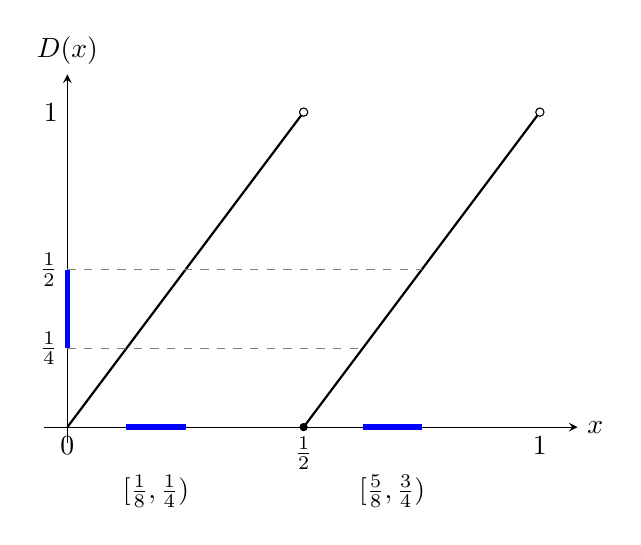
\begin{tikzpicture}[x=6cm,y=4cm,>=stealth]
 \draw[->] (-.05,0)--(1.08,0) node[right]{\(x\)};
 \draw[->] (0,-.05)--(0,1.12) node[above]{\(D(x)\)};
 \draw[thick] (0,0)--(.5,1);
 \draw[thick] (.5,0)--(1,1);
 \draw[fill=white] (.5,1) circle[radius=1.5pt];
 \draw[fill=white] (1,1) circle[radius=1.5pt];
 \fill (.5,0) circle[radius=1.5pt];
 \draw[dashed,gray] (0,.25)--(.625,.25);
 \draw[dashed,gray] (0,.5)--(.75,.5);
 \draw[line width=2pt,blue] (0,.25)--(0,.5);
 \draw[line width=2pt,blue] (.125,0)--(.25,0);
 \draw[line width=2pt,blue] (.625,0)--(.75,0);
 \node[left] at (0,.25){\(\frac14\)};
 \node[left] at (0,.5){\(\frac12\)};
 \node[left] at (0,1){\(1\)};
 \node[below] at (0,0){\(0\)};
 \node[below] at (.5,0){\(\frac12\)};
 \node[below] at (1,0){\(1\)};
 \node[below] at (.1875,-.12){\([\frac18,\frac14)\)};
 \node[below] at (.6875,-.12){\([\frac58,\frac34)\)};
\end{tikzpicture}
\caption[倍增映射及区间的两个逆像]{倍增映射及区间的两个逆像。
蓝色目标区间为 \([1/4,1/2)\)，其两个逆像各长 \(1/8\)，总长仍为 \(1/4\)。
分支顶端的空心点表示该端点不属于相应分支。}
\label{b1:fig:doubling-map-32}
\end{figure}

迭代 \(n\) 次后，\(D^n(x)=2^nx\bmod1\) 有 \(2^n\) 个这样的分支。
每个长度 \(2^{-n}\) 的二进区间都被拉伸为整个 \([0,1)\)。
因此，一个只分辨到较粗二进尺度的初始事件，
在足够晚的时刻会与任意固定目标事件精确独立，而不仅仅是近似独立。

\begin{lemma}[二进区间上的精确相关]
\label{b1:lem:dyadic-independence-32}
设 \(D(x)=2x\bmod1\) 作用于 \([0,1)\) 上的 Borel 概率空间与长度测度 \(m\)。
对整数 \(r\geq0\)、\(0\leq j<2^r\)，令
\[
 I_{r,j}=[j2^{-r},(j+1)2^{-r}).
\]
则对任意 Borel 集 \(B\subseteq[0,1)\) 以及整数 \(n\geq r\)，
\[
 m(I_{r,j}\cap D^{-n}B)=2^{-r}m(B).
\]
若 \(A\) 是若干个同级 \(I_{r,j}\) 的并，则
\(m(A\cap D^{-n}B)=m(A)\cdot m(B)\) 对 \(n\geq r\) 成立。
\end{lemma}
\begin{proof}
把 \(I_{r,j}\) 划分成 \(2^{n-r}\) 个 \(n\) 级区间
\(J_\ell=[\ell2^{-n},(\ell+1)2^{-n})\)。
在每个 \(J_\ell\) 上，\(D^n(x)=2^nx-\ell\)，
故 \(J_\ell\cap D^{-n}B=(B+\ell)/2^n\)，其测度为 \(2^{-n}m(B)\)。
把这些互不相交的部分相加，得到
\(2^{n-r}\cdot2^{-n}m(B)=2^{-r}m(B)\)。
若 \(A\) 含有多个 \(r\) 级区间，再利用有限可加性即可。
\end{proof}

\begin{theorem}[倍增映射的混合性]
\label{b1:thm:doubling-mixing-32}
区间 \([0,1)\) 上的倍增映射 \(D(x)=2x\bmod1\)
关于 Borel \(\sigma\)-代数及长度概率测度 \(m\) 是混合的，因而是遍历的。
\end{theorem}
\begin{proof}
保测性已在\secref{b1:sec:3201}证明。
取任意 Borel 集 \(A,B\subseteq[0,1)\) 及 \(\varepsilon>0\)。
可以用某一级二进区间的有限并 \(A_r\) 使 \(m(A\triangle A_r)<\varepsilon\)：
先用有限个普通区间逼近 \(A\)，再把有限多个端点分别移到足够细的二进网格上。
若共有 \(s\) 个区间，后一步造成的对称差至多为 \(2s\,2^{-r}\)。

对每个 \(n\geq r\)，上一引理给出
\(m(A_r\cap D^{-n}B)=m(A_r)\cdot m(B)\)。从而
\[
 \begin{aligned}
 &|m(A\cap D^{-n}B)-m(A)\cdot m(B)|\\
 &\leq|m(A\cap D^{-n}B)-m(A_r\cap D^{-n}B)|
       +|m(A_r)-m(A)|\cdot m(B)\\
 &\leq2m(A\triangle A_r)<2\varepsilon.
 \end{aligned}
\]
第一项只在 \(A\triangle A_r\) 内可能发生变化。
固定 \(\varepsilon\) 所对应的 \(r\)，再让 \(n\to\infty\)，就得到混合性；
由\cref{b1:prop:mixing-ergodic-32}得到遍历性。
\end{proof}

二进制展开能解释上面的分支计算。
除去有两个二进制展开的可数个二进有理数，写
\[
 x=0.\xi_1\xi_2\xi_3\cdots\quad(\xi_j\in\{0,1\}),
\]
则 \(D\) 抹去第一位，\(D^n\) 抹去前 \(n\) 位。
指定前 \(r\) 位就是指定一个长度 \(2^{-r}\) 的区间。
当 \(n\geq r\) 时，这些已知的前位与 \(n\) 步后的尾部互不重叠；
前一引理用长度计算证明了相应独立性，而不要求读者先接受“二进位天然独立”。

\ProseParagraphBreak

取 \(f=\mathbf1_{[0,1/2)}\)，由\cref{b1:cor:ergodic-time-space-32}和
\cref{b1:thm:doubling-mixing-32}，对几乎每个 \(x\)，前 \(N\) 个二进位中零的比例趋于 \(1/2\)。
固定点 \(x=0\) 却始终给出比例一；它所在的单点是零测集，并不违反定理。
同样，上一节 \(L^\infty\) 反例中的正测度小区间
\([0,2^{-N})\) 正是前 \(N\) 位全为零的起点集合。
因此混合、逐点几乎处处收敛和不具有 \(L^\infty\) 范数收敛，
可以在同一个简单系统中同时出现。

\ProseParagraphBreak

本章的两个圆周模型使用同一长度概率测度，却呈现不同的长期相关。
无理转动保留相位，时间平均靠抵消稳定下来；
倍增映射把有限尺度的信息不断移到更远的二进位，固定事件间的相关因而消失。
两者都不需要一般谱表示或独立同分布极限定理作为前提。
熵、弱混合以及一般遍历分解将进一步区分动力系统，本章所证的范围止于这里。


\begin{chaptersummary}
保测性使 \(f\) 与 \(f\circ T\) 具有相同的积分和 \(L^p\) 范数，
但轨道仍可能被限制在不同的不变部分之中。
模零不变子代数把这些不能由时间演化消除的信息集中起来；
遍历性表示其中每个事件的概率都是零或一，而不是要求每条轨道都逐点访问整个空间。

\ProseParagraphBreak

在 Hilbert 空间中，平均收敛来自一个正交分解。
固定向量在平均下保持不动；形如 \(g-Ug\) 的向量逐项相消，平均趋于零。
收缩性使这个结论能推广到算子差值域的闭包。
对保测系统的 Koopman 算子，保留下来的正交投影正是相对于不变信息的条件平均。

\ProseParagraphBreak

逐点收敛需要比范数逼近更多的控制。
Hopf 极大引理估计所有长度上发生越界的集合，
使有界不变函数与有界差分组成的稠密类能够控制一般可积函数的振幅。
Birkhoff 定理随后把有限的逐点极限识别为 \(\mathbb E_\mu(f\mid\mathcal I_T)\)，
并在概率空间上同时给出 \(L^1\) 收敛。
若 \(f\in L^p\)、\(1\leq p<\infty\)，还得到相应的 \(L^p\) 收敛；
不能由此把端点 \(p=\infty\) 的范数收敛也一并写入结论。

\ProseParagraphBreak

遍历时，不变信息中的条件平均退化成空间积分；混合性进一步要求远隔时刻的相关趋于独立乘积。
无理圆周转动遍历而不混合，二进倍增映射则具有混合性。
这两个模型说明，轨道平均的存在、平均是否为常数、相关是否消失，各有自己的条件和证明。
它们把测度的保持、函数空间中的投影和几乎处处的轨道行为连接起来，也保留了三者之间需要辨认的边界。
\end{chaptersummary}

\BookExercises

% 目标：检验保测假设不可删，并区分参考测度与变换自身的不变概率。
% 来源：自拟；以收缩映射作完整反例，不改编外部习题。
\begin{exercise}\label{b1:ex:32-nonpreserving-contraction}
在 \([0,1]\) 的 Borel \(\sigma\)-代数上取 Lebesgue 概率测度 \(m\)，令 \(T(x)=x/2\)。
证明 \(T\) 不保持 \(m\)，但对每个实或复连续函数 \(f\in C([0,1])\)，都有
\[
 A_nf(x)=\frac1n\sum_{k=0}^{n-1}f(T^kx)\longrightarrow f(0)
 \quad\text{在 }[0,1]\text{ 上一致成立}.
\]
用 \(f(x)=x\) 比较这个极限与 \(\int_0^1f\,\mathrm dx\)。
进一步证明，\(\delta_0\) 是 \(T\) 在 \([0,1]\) 上唯一的不变 Borel 概率测度，
其中 \(\delta_0(A)=\mathbf1_A(0)\)。
\end{exercise}
\begin{solution}
取 \(A=[0,1/2]\)。由于 \(T^{-1}A=[0,1]\)，有
\(m(T^{-1}A)=1\)，而 \(m(A)=1/2\)，所以 \(T\) 不保 \(m\)。

连续函数在紧区间上有界，而且在 \(0\) 处连续。
给定 \(\varepsilon>0\)，可取整数 \(K\geq1\)，使
\(0\leq y\leq2^{-K}\) 时 \(|f(y)-f(0)|<\varepsilon\)。
当 \(k\geq K\) 时，对所有 \(x\in[0,1]\) 都有 \(T^kx=x/2^k\leq2^{-K}\)。
因此对 \(n>K\)，
\[
 \sup_{x\in[0,1]}|A_nf(x)-f(0)|
 \leq\frac{2K\|f\|_\infty}{n}+\varepsilon.
\]
先令 \(n\to\infty\)，再令 \(\varepsilon\downarrow0\)，便得一致收敛。
特别地，\(f(x)=x\) 时极限为零，空间积分却是 \(1/2\)。
轨道越来越接近零点，不能代表 Lebesgue 测度在整个区间上的分布。

因为 \(T(0)=0\)，\(\delta_0(T^{-1}A)=\delta_0(A)\)，故 \(\delta_0\) 不变。
若 \(\nu\) 是任意不变 Borel 概率测度，则保测性的积分形式用于有界函数 \(x\mapsto x\)，得到
\[
 \int_{[0,1]}x\,\mathrm d\nu
 =\int_{[0,1]}T(x)\,\mathrm d\nu
 =\frac12\int_{[0,1]}x\,\mathrm d\nu.
\]
故该非负积分为零。对每个 \(j\geq1\)，
\(\nu([1/j,1])\leq j\int x\,\mathrm d\nu=0\)，
再对这些集合取并，得到 \(\nu((0,1])=0\)。
概率的全部质量只能位于 \(0\)，所以 \(\nu=\delta_0\)。
相对于这一不变概率，前面的时间极限确实就是空间积分；失败的是把任意指定的参考测度当作不变测度。
\end{solution}

% 目标：从有限总质量证明几乎处处反复回返，涵盖不可逆变换并检验有限性。
% 来源：自拟；完整重建回归论证，正文不以本题为前置。
\begin{exercise}[Poincaré 回归]\label{b1:ex:32-poincare-recurrence}
设 \((X,\mathcal A,\mu)\) 为概率空间，\(T:X\to X\) 为可测保测变换，\(A\in\mathcal A\)。
证明对几乎每个 \(x\in A\)，存在无穷多个正整数 \(n\) 使 \(T^nx\in A\)。
这一结论称为\term[poincare-huigui-dingli]{Poincaré 回归定理}[Poincaré recurrence theorem]。
证明不得假设 \(T\) 可逆。
再在带计数测度的 \(\mathbb Z\) 上给出一个可逆保测变换和一个正测度集合，
说明无限测度空间中相同断言可以失败。
\end{exercise}
\begin{solution}
先考虑离开以后再也不回来的点所成的集合
\[
 W=A\cap\bigcap_{n=1}^\infty T^{-n}(X\setminus A).
\]
集合 \(T^{-j}W\)、\(j\geq0\) 两两不交。
事实上，若 \(j<k\) 且 \(x\) 同时属于 \(T^{-j}W\) 与 \(T^{-k}W\)，
则 \(y=T^jx\in W\subset A\)，同时 \(T^{k-j}y\in W\subset A\)，
这与 \(W\) 中的点在正时间不再进入 \(A\) 矛盾。
保测性给出 \(\mu(T^{-j}W)=\mu(W)\)，故对每个 \(N\geq0\)，
\[
 (N+1)\cdot\mu(W)
 =\mu\left(\bigcup_{j=0}^NT^{-j}W\right)\leq1.
\]
令 \(N\to\infty\)，得到 \(\mu(W)=0\)。

若 \(x\in A\) 只在有限多个正时间回到 \(A\)，
那么包括初始时刻 \(0\) 在内，它必有一个最后进入 \(A\) 的时刻 \(j\geq0\)。
这时 \(T^jx\in W\)，所以所有这样的 \(x\) 都属于
\(\bigcup_{j\geq0}T^{-j}W\)。
该集合的测度为零，便得到所需的无限次回返。
证明中只用到了原像及正向迭代，没有用到逆映射。

最后在 \(\mathbb Z\) 的全部子集上取计数测度，令 \(T(k)=k+1\)、\(A=\{0\}\)。
平移为双射，保持集合的元素个数，因而保测；但 \(T^n(0)=n\notin A\) 对每个 \(n\geq1\) 成立。
此时那些互不相交的原像都具有测度一，总质量却允许为无穷，前面的有限总质量论证不再适用。
回归结论只保证反复进入，不为第一次回返提供统一的时间上界。
\end{solution}

% 目标：用逐点遍历极限比较不同不变概率，并检验绝对连续性的作用。
% 来源：自拟；把Birkhoff定理连接到测度唯一性，不假设密度逐点不变。
\begin{exercise}\label{b1:ex:32-absolutely-continuous-invariant-probability}
设 \((X,\mathcal A,\mu)\) 为概率空间，\(T:X\to X\) 为可测、保 \(\mu\) 且遍历的变换。
设 \(\nu\) 是 \((X,\mathcal A)\) 上另一概率测度，满足
\[
 \nu\ll\mu,
 \quad\nu(T^{-1}A)=\nu(A)\quad(A\in\mathcal A).
\]
证明 \(\nu=\mu\)。
再用 \([0,1)\) 上的倍增映射 \(D(x)=2x-\lfloor2x\rfloor\)，
说明若删去绝对连续条件，即使 \(\mu\) 下的系统具有混合性，不变概率也未必唯一。
\end{exercise}
\begin{solution}
固定 \(A\in\mathcal A\)。由于 \(\mathbf1_A\) 有界可积，
Birkhoff 定理\cref{b1:thm:birkhoff-32}及遍历性给出
\[
 \frac1n\sum_{k=0}^{n-1}\mathbf1_A(T^kx)\longrightarrow\mu(A)
 \quad\text{对 }\mu\text{-几乎每个 }x.
\]
绝对连续性 \(\nu\ll\mu\) 保证同一极限也在 \(\nu\)-几乎处处成立。
每个平均都位于 \([0,1]\)，而 \(\nu\) 是概率测度，
所以相对于 \(\nu\) 可以用常数 \(1\) 作支配函数并交换积分与极限。
另一方面，\(\nu\) 的不变性给出
\[
 \int_X\frac1n\sum_{k=0}^{n-1}\mathbf1_A\circ T^k\,\mathrm d\nu
 =\frac1n\sum_{k=0}^{n-1}\nu(T^{-k}A)=\nu(A).
\]
令 \(n\to\infty\)，左侧趋于 \(\mu(A)\)，于是 \(\nu(A)=\mu(A)\)。
因为 \(A\) 任意，两个测度相等。
绝对连续性把 \(\mu\)-零测的轨道例外集仍视为 \(\nu\)-零测。

对倍增映射，\cref{b1:thm:doubling-mixing-32}说明 Lebesgue 概率测度 \(m\) 不变且系统混合。
但 \(D(0)=0\)，所以集中在零点的 \(\delta_0\) 也是不变概率。
二者不同，且 \(m(\{0\})=0\)、\(\delta_0(\{0\})=1\)，恰好违反绝对连续条件。
本题的唯一性只在相对于给定遍历概率绝对连续的不变概率类中成立。
\end{solution}

% 目标：把遍历定理用于有重叠的有限字串频率，并处理可数个字串的共同例外集。
% 来源：自拟；正文仅讨论单个二进数字，本题推广到任意有限字。
\begin{exercise}\label{b1:ex:32-binary-word-frequencies}
在 \([0,1)\) 的 Borel \(\sigma\)-代数上取 Lebesgue 概率测度 \(m\)。
除去形如 \(k/2^s\) 的二进有理数后，每个点都有唯一的展开
\[
 x=\sum_{j=1}^\infty\varepsilon_j(x)\,2^{-j},
 \quad\varepsilon_j(x)\in\{0,1\}.
\]
设 \(r\geq1\)，\(w=(w_1,\ldots,w_r)\in\{0,1\}^r\) 为固定有限字。
证明对几乎每个 \(x\)，
\[
 \frac1N\#\{\,0\leq k<N:
       (\varepsilon_{k+1}(x),\ldots,\varepsilon_{k+r}(x))=w\,\}
 \longrightarrow 2^{-r}.
\]
证明可选同一个满测度集合，使该结论对所有 \(r\) 与所有 \(w\) 同时成立。
若只统计完全位于前 \(N\) 个数字之内的出现次数，说明极限为何仍相同。
\end{exercise}
\begin{solution}
记 \(j(w)=\sum_{i=1}^r w_i2^{r-i}\)，并取半开二进区间
\[
 J_w=\left[\frac{j(w)}{2^r},\frac{j(w)+1}{2^r}\right).
\]
除去二进有理数后，\(x\in J_w\) 当且仅当它的前 \(r\) 个二进数字恰为 \(w\)。
倍增映射 \(D(x)=2x-\lfloor2x\rfloor\) 把第一个数字移去，
故题中的次数正是
\[
 \sum_{k=0}^{N-1}\mathbf1_{J_w}(D^kx).
\]
二进有理数构成可数集，测度为零；非二进有理数经任意次倍增后仍不是二进有理数，
所以这里不会沿轨道再遇到展开歧义。

由\cref{b1:thm:doubling-mixing-32}，\(D\) 保测且混合，因而遍历。
对有界可积函数 \(\mathbf1_{J_w}\) 使用\cref{b1:thm:birkhoff-32}，便得到几乎处处的极限
\(m(J_w)=2^{-r}\)。
对每个 \(r\) 只有 \(2^r\) 个字，而 \(r\) 只取正整数，因此所有有限二进字总共可数。
把各字所需排除的零测集与二进有理数集取可数并，余下便是使全部结论同时成立的满测度集合。

若只统计前 \(N\) 个数字中完整出现的字，则对 \(N\geq r\)，起点只能取
\(k=0,\ldots,N-r\)。这与原计数至多相差最后 \(r-1\) 个起点；
除以 \(N\) 后差至多为 \((r-1)/N\)，趋于零。
若改以可用起点数 \(N-r+1\) 作分母，因 \((N-r+1)/N\to1\)，极限也不改变。
相邻字串可能共享多个数字，因而相应示性函数并不独立；
这些计数可能重叠，遍历性仍能确定它们的长期频率。
\end{solution}

% 目标：区分零条件平均、差分值域及其闭包；用能量增长排除L2差分表示。
% 来源：自拟；增加正文稠密分解没有给出的非闭值域实例。
\begin{exercise}[零平均与差分表示]\label{b1:ex:32-zero-mean-not-difference}
在 \([0,1)\) 的 Borel \(\sigma\)-代数上取 Lebesgue 概率测度 \(m\)，令
\[
 D(x)=2x-\lfloor2x\rfloor,
 \quad f=\mathbf1_{[0,1/2)}-\mathbf1_{[1/2,1)}.
\]
证明 \(\int_0^1 f\,\mathrm dm=0\)，并且对每个整数 \(N\geq1\)，
\[
 \left\|\sum_{k=0}^{N-1}f\circ D^k\right\|_2^2=N.
\]
由此证明不存在实或复函数 \(g\in L^2(m)\) 满足
\(f=g-g\circ D\) 几乎处处。
解释这一结论为何不与平均遍历定理中的正交分解矛盾。
\end{exercise}
\begin{solution}
两个半区间的测度都是 \(1/2\)，所以 \(f\) 的积分为零，且 \(f^2=1\) 处处成立。
令 \(Z_k=f\circ D^k\)。保测性给出 \(\|Z_k\|_2^2=1\)。
若 \(0\leq j<k\)，用长度为 \(2^{-(k+1)}\) 的半开二进区间分割 \([0,1)\)。
在这些区间上，前 \(k+1\) 位数字遍取所有 \(2^{k+1}\) 种模式，且各模式的测度相同。
二进展开有歧义的点只有可数个，不影响下面的积分。
\(Z_j\) 只取决于第 \(j+1\) 位，\(Z_k\) 只取决于第 \(k+1\) 位；
这两位的四种组合各出现 \(2^{k-1}\) 次。
因此乘积 \(Z_jZ_k\) 取 \(1\)、\(-1\) 的集合测度各为 \(1/2\)，有
\(\int Z_jZ_k\,\mathrm dm=0\)。
展开平方并积分便得
\[
 \left\|\sum_{k=0}^{N-1}Z_k\right\|_2^2
 =\sum_{k=0}^{N-1}\|Z_k\|_2^2
  +2\sum_{0\leq j<k<N}\int Z_jZ_k\,\mathrm dm=N.
\]

假设 \(f=g-g\circ D\) 且 \(g\in L^2(m)\)。
由于 \(D\) 保持零测集的原像，逐次复合的等式仍在 \(L^2\) 中成立。
有限项相消给出
\[
 \sum_{k=0}^{N-1}f\circ D^k=g-g\circ D^N.
\]
保测性又给出 \(\|g\circ D^N\|_2=\|g\|_2\)，于是
\(\sqrt N\leq2\|g\|_2\) 对所有 \(N\) 成立，矛盾。
对复值 \(g\)，相同的范数估计仍成立，所以也不可能。

倍增系统遍历，故 \(L^2\) 中不变子空间由常数构成。
本题的 \(f\) 与所有常数正交，按平均遍历定理的分解，它属于
\(\overline{\operatorname{Ran}(I-U)}\)，其中 \(Ug=g\circ D\)。
该分解写的是值域的闭包，并没有断言 \(f\) 本身就是一个差分。
实际上，\(\|A_Nf\|_2=N^{-1/2}\to0\)，
平均仍然收敛，而未除以 \(N\) 的部分和却不可能一致有界于 \(L^2\)。
这正体现了闭包与原值域之间的差别。
\end{solution}

% 目标：区分固定事件的混合极限与对全部事件同时取上确界，并求出界的精确值。
% 来源：自拟；通过随时间移动的事件建立量词反例。
\begin{exercise}\label{b1:ex:32-mixing-not-uniform-in-events}
在 \([0,1)\) 的 Borel \(\sigma\)-代数 \(\mathcal B\) 上取 Lebesgue 概率测度 \(m\)，
令 \(D(x)=2x-\lfloor2x\rfloor\)。证明对每个整数 \(n\geq1\)，
\[
 \sup_{A,B\in\mathcal B}
 \bigl|m(D^{-n}A\cap B)-m(A)\cdot m(B)\bigr|=\frac14.
\]
解释为什么这不与 \(D\) 的混合性矛盾。
\end{exercise}
\begin{solution}
取任意 \(A,B\in\mathcal B\)，记 \(a=m(A)\)、\(b=m(B)\)。
由于 \(D\) 保测，\(m(D^{-n}A)=a\)。将相关差写成两个中心化示性函数的乘积积分，得到
\[
 \begin{aligned}
 &m(D^{-n}A\cap B)-ab\\
 &\quad=\int_0^1(\mathbf1_{D^{-n}A}-a)
                     (\mathbf1_B-b)\,\mathrm dm.
 \end{aligned}
\]
Cauchy--Schwarz 不等式给出绝对值至多为
\(\sqrt{a(1-a)b(1-b)}\leq1/4\)，因为 \(t(1-t)\leq1/4\) 对 \(0\leq t\leq1\) 成立。

反过来，固定 \(A=[0,1/2)\)，并针对给定 \(n\) 选 \(B_n=D^{-n}A\)。
这时 \(m(A)=m(B_n)=1/2\)，且 \(D^{-n}A\cap B_n=B_n\)，所以相关差为
\(1/2-1/4=1/4\)。这既达到上界，也证明了等式。

混合性先固定一对事件 \(A,B\)，再令 \(n\to\infty\)。
本题则在每个 \(n\) 重新选择 \(B_n\)，故所考察的不是同一对事件之间随时间消失的相关。
不同事件对所需的等待时间可以不同；逐对收敛不提供对所有事件共同有效的误差界。
\end{solution}

% 目标：构造两个遍历系统之积不遍历的例子，并通过坐标变换显式计算不变条件平均。
% 来源：自拟；以对角转动训练Fubini、模零不变性及条件期望的结合。
\begin{optionalexercise}\label{b1:ex:32-product-rotations}
记 \(\mathbb T=\mathbb R/\mathbb Z\)，其 Borel \(\sigma\)-代数上的归一化 Lebesgue 测度为 \(m\)。
固定无理数 \(\alpha\)，在概率空间 \((\mathbb T^2,\mathcal B(\mathbb T^2),m\otimes m)\) 上令
\[
 T(x,y)=(x+\alpha,y+\alpha),
\]
坐标加减均按模 \(1\) 理解。证明每个单独的圆周转动 \(x\mapsto x+\alpha\) 都遍历，
但乘积变换 \(T\) 不遍历。证明 \(T\) 的不变事件模零恰好由差坐标 \(y-x\) 决定。
对实或复函数 \(f\in L^1(m\otimes m)\)，证明
\[
 \frac1n\sum_{k=0}^{n-1}f(x+k\alpha,y+k\alpha)
 \longrightarrow\int_0^1f(x+t,y+t)\,\mathrm dt
\]
对 \(m\otimes m\)-几乎每个 \((x,y)\) 成立，并且在 \(L^1\) 中成立。
说明右侧为什么存在于几乎每个点，以及它与条件期望的关系。
\end{optionalexercise}
\begin{solution}
单个无理转动的遍历性已由\cref{b1:thm:irrational-rotation-32}证明。
转动保持圆周测度，因而乘积变换保持乘积测度；也可逐变量积分核对这一点。
但差坐标满足 \((y+\alpha)-(x+\alpha)=y-x\)，故事件
\[
 E=\{\,(x,y):y-x\in[0,1/2)\,\}
\]
不变且具有测度 \(1/2\)。因此 \(T\) 不遍历。

要辨认全部不变信息，作坐标变换
\[
 S(x,y)=(u,v)=(x,y-x),
 \quad S^{-1}(u,v)=(u,u+v).
\]
它是 Borel 双射且保持乘积测度。
事实上，对任意非负 Borel 函数 \(F\)，先固定 \(u\)，利用圆周平移不改变 \(m\)，
再用 Tonelli 定理，有
\[
 \int_{\mathbb T^2}F(x,y-x)\,\mathrm d(m\otimes m)
 =\int_{\mathbb T}\int_{\mathbb T}F(u,v)\,\mathrm dm(v)\,\mathrm dm(u).
\]
在这些坐标中，\(STS^{-1}(u,v)=(u+\alpha,v)\)。

设 \(A\) 为模零不变的 Borel 事件，记 \(H=\mathbf1_A\circ S^{-1}\)。
模零不变性意味着 \(H(u+\alpha,v)=H(u,v)\) 在乘积测度下几乎处处成立。
由 Fubini 定理，对几乎每个 \(v\)，此等式关于 \(u\) 几乎处处成立。
无理转动遍历，所以这个 \(\{0,1\}\)-值不变函数关于 \(u\) 几乎处处为常数。
令 \(p(v)=\int_{\mathbb T}H(u,v)\,\mathrm dm(u)\)，则 \(p\) 可测且几乎处处只取 \(0\) 或 \(1\)。
取 Borel 集 \(B=\{v:p(v)>1/2\}\)，便有 \(H(u,v)=\mathbf1_B(v)\) 几乎处处。
反过来，任何只依赖 \(v\) 的事件都不变。
回到原坐标，便证明不变事件模零恰好由 \(y-x\) 决定。

现取 \(f\in L^1(m\otimes m)\) 的可测代表。保测坐标变换与 Fubini 定理保证
\[
 G(v)=\int_{\mathbb T}f(u,u+v)\,\mathrm dm(u)
\]
对几乎每个 \(v\) 绝对收敛，并且 \(G\in L^1(m)\)；在其余可测零测集上令 \(G=0\)。
于是 \(g(x,y)=G(y-x)\) 可积且为不变子代数可测。
对任何 Borel 集 \(B\subset\mathbb T\)，Fubini 定理给出
\[
 \int_{\{y-x\in B\}}f\,\mathrm d(m\otimes m)
 =\int_B G\,\mathrm dm
 =\int_{\{y-x\in B\}}g\,\mathrm d(m\otimes m).
\]
因为全部不变事件都模零具有这种形式，条件期望的积分刻画说明
\(g=\mathbb E(f\mid\mathcal I_T)\)。
令 \(u=x+t\)，圆周平移保持积分，故对几乎每个 \((x,y)\)，
\(G(y-x)=\int_0^1 f(x+t,y+t)\,\mathrm dt\)。
最后使用\cref{b1:thm:birkhoff-32}，即得题中的几乎处处收敛与 \(L^1\) 收敛。
空间积分还会再平均差坐标 \(v\)，单条对角轨道却始终保留它；两者不能在此模型中混为一个常数。
\end{solution}

% 目标：检验遍历性对幂迭代的稳定性，用有限周期结构计算失去的信息。
% 来源：自拟；一般k/r必要条件加可核算模型，不引入一般因子分类。
\begin{optionalexercise}\label{b1:ex:32-powers-periodic-factor}
设 \((X,\mathcal A,\mu)\) 为概率空间，\(T:X\to X\) 为可测保测且遍历的变换，
整数 \(r\geq2\)。若 \(A\in\mathcal A\) 满足 \(\mu(T^{-r}A\mathbin{\triangle}A)=0\)，证明
\[
 \mu(A)\in\left\{0,\frac1r,\frac2r,\ldots,1\right\}.
\]
再令 \(\mathbb T=\mathbb R/\mathbb Z\)，其 Borel \(\sigma\)-代数上的归一化 Lebesgue 测度为 \(m\)。
在 \(X=\{0,\ldots,r-1\}\times\mathbb T\) 的乘积 \(\sigma\)-代数上，
取有限集上的均匀概率与 \(m\) 的乘积概率 \(\mu\)。固定无理数 \(\alpha\)，定义
\[
 T(j,x)=(j+1\bmod r,x+\alpha).
\]
证明 \(T\) 遍历，而 \(T^r\) 不遍历；证明 \(T^r\) 的不变事件模零恰为若干整分量
\(\{j\}\times\mathbb T\) 的并。对任意实或复 \(f\in L^1(\mu)\)，分别求沿 \(T\) 与 \(T^r\) 的时间平均极限。
\end{optionalexercise}
\begin{solution}
对一般系统，令
\[
 h=\sum_{j=0}^{r-1}\mathbf1_A\circ T^j.
\]
因为 \(\mathbf1_A\circ T^r=\mathbf1_A\) 几乎处处，逐项相减得到
\(h\circ T-h=\mathbf1_A\circ T^r-\mathbf1_A=0\) 几乎处处。
函数 \(h\) 有界、不变，故由遍历性的函数判别\cref{b1:prop:ergodicity-criterion-32}，
它几乎处处等于某个常数 \(c\)。又因 \(h\) 只取整数 \(0,\ldots,r\)，
该常数也是这些整数之一。保测性给出
\[
 c=\int_Xh\,\mathrm d\mu=r\cdot\mu(A),
\]
从而得到所需的取值限制。它并不排除 \(1/r\) 等中间值，因而尚不能说明 \(T^r\) 遍历。

在题给模型中，有限坐标的循环置换与圆周平移都保各自的概率，故 \(T\) 保测。
直接迭代得到 \(T^r(j,x)=(j,x+r\alpha)\)。
因为 \(r\alpha\) 仍为无理数，\cref{b1:thm:irrational-rotation-32}说明
每个分量上的 \(T^r\) 都是遍历的无理转动。
若事件 \(A\) 对 \(T^r\) 模零不变，则其每个截面
\(A_j=\{x:(j,x)\in A\}\) 对该转动模零不变，故每个 \(m(A_j)\) 只能为零或一。
由于只有有限个截面，\(A\) 模零等于那些满足 \(m(A_j)=1\) 的整分量之并。
反过来，整分量的并在 \(T^r\) 下确实不变。
特别地，单个分量的测度为 \(1/r\)，所以 \(T^r\) 不遍历。

若 \(A\) 对 \(T\) 模零不变，则由保测性，反复取原像并取有限个零测例外集的并，
可知它也对 \(T^r\) 模零不变。因此它模零由一些整分量构成。
而 \(T\) 循环移动这些分量，\(T\)-不变性迫使每个分量的选择相同：全部选择或全部舍弃。
故 \(\mu(A)=1\) 或 \(0\)，证明 \(T\) 遍历。

最后，对 \(f\in L^1(\mu)\)，每个截面 \(f(j,\cdot)\) 都可积，
因为有限个非负截面积分的平均有限。
沿 \(T\) 的平均由 Birkhoff 定理趋于常数
\[
 \int_Xf\,\mathrm d\mu
 =\frac1r\sum_{j=0}^{r-1}\int_{\mathbb T}f(j,x)\,\mathrm dm(x).
\]
沿 \(T^r\) 的平均则在第 \(j\) 个分量上趋于
\[
 g(j,x)=\int_{\mathbb T}f(j,y)\,\mathrm dm(y).
\]
两种收敛均在 \(\mu\)-几乎处处及 \(L^1(\mu)\) 中成立。
后一函数正是给定有限坐标 \(j\) 后的条件平均。
每隔 \(r\) 步观察一次，恰好使有限坐标保持不动，因而保留了逐步观察时会被平均掉的分量信息。
\end{solution}
